%Block 5: Techniken und Methoden
\begin{frame}{Gute Lötstelle}
\begin{columns}[T]
    \begin{column}{0.58\textwidth}
        \small
        \begin{itemize}\setlength{\itemsep}{3mm}
            \item Eine gute Lötstelle wirkt \textbf{leicht glänzend} und \textbf{gleichmäßig}.
            \item Das Lot sollte \textbf{sauber um Pin und Pad} fließen und eine ruhige Form bilden.
            \item Es dürfen keine \textbf{Brücken} entstehen und die Verbindung sollte \textbf{mechanisch fest} sein.
        \end{itemize}
        \normalsize
    \end{column}
    \begin{column}{0.42\textwidth}
        \centering
        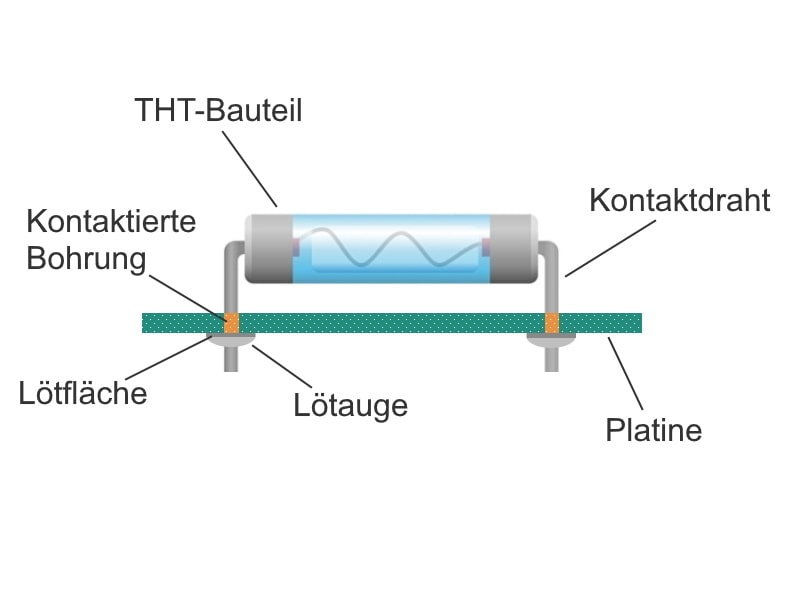
\includegraphics[width=\linewidth,keepaspectratio]{2.0.0.0_content/assets/bilder/tht_löten.jpg}
    \end{column}
\end{columns}
\end{frame}

\begin{frame}{Vorbereitung}
\begin{columns}[T]
    \begin{column}{0.58\textwidth}
        \small
        \begin{itemize}\setlength{\itemsep}{3mm}
            \item Das \textbf{Bauteil einsetzen} und die Beinchen leicht spreizen, damit es nicht herausfällt.
            \item Die \textbf{Spitze reinigen} und kurz mit etwas Lot benetzen.
            \item \textbf{Kontaktflächen sauber halten} und das Werkstück möglichst ruhig fixieren.
        \end{itemize}
        \normalsize
    \end{column}
    \begin{column}{0.42\textwidth}
        \centering
        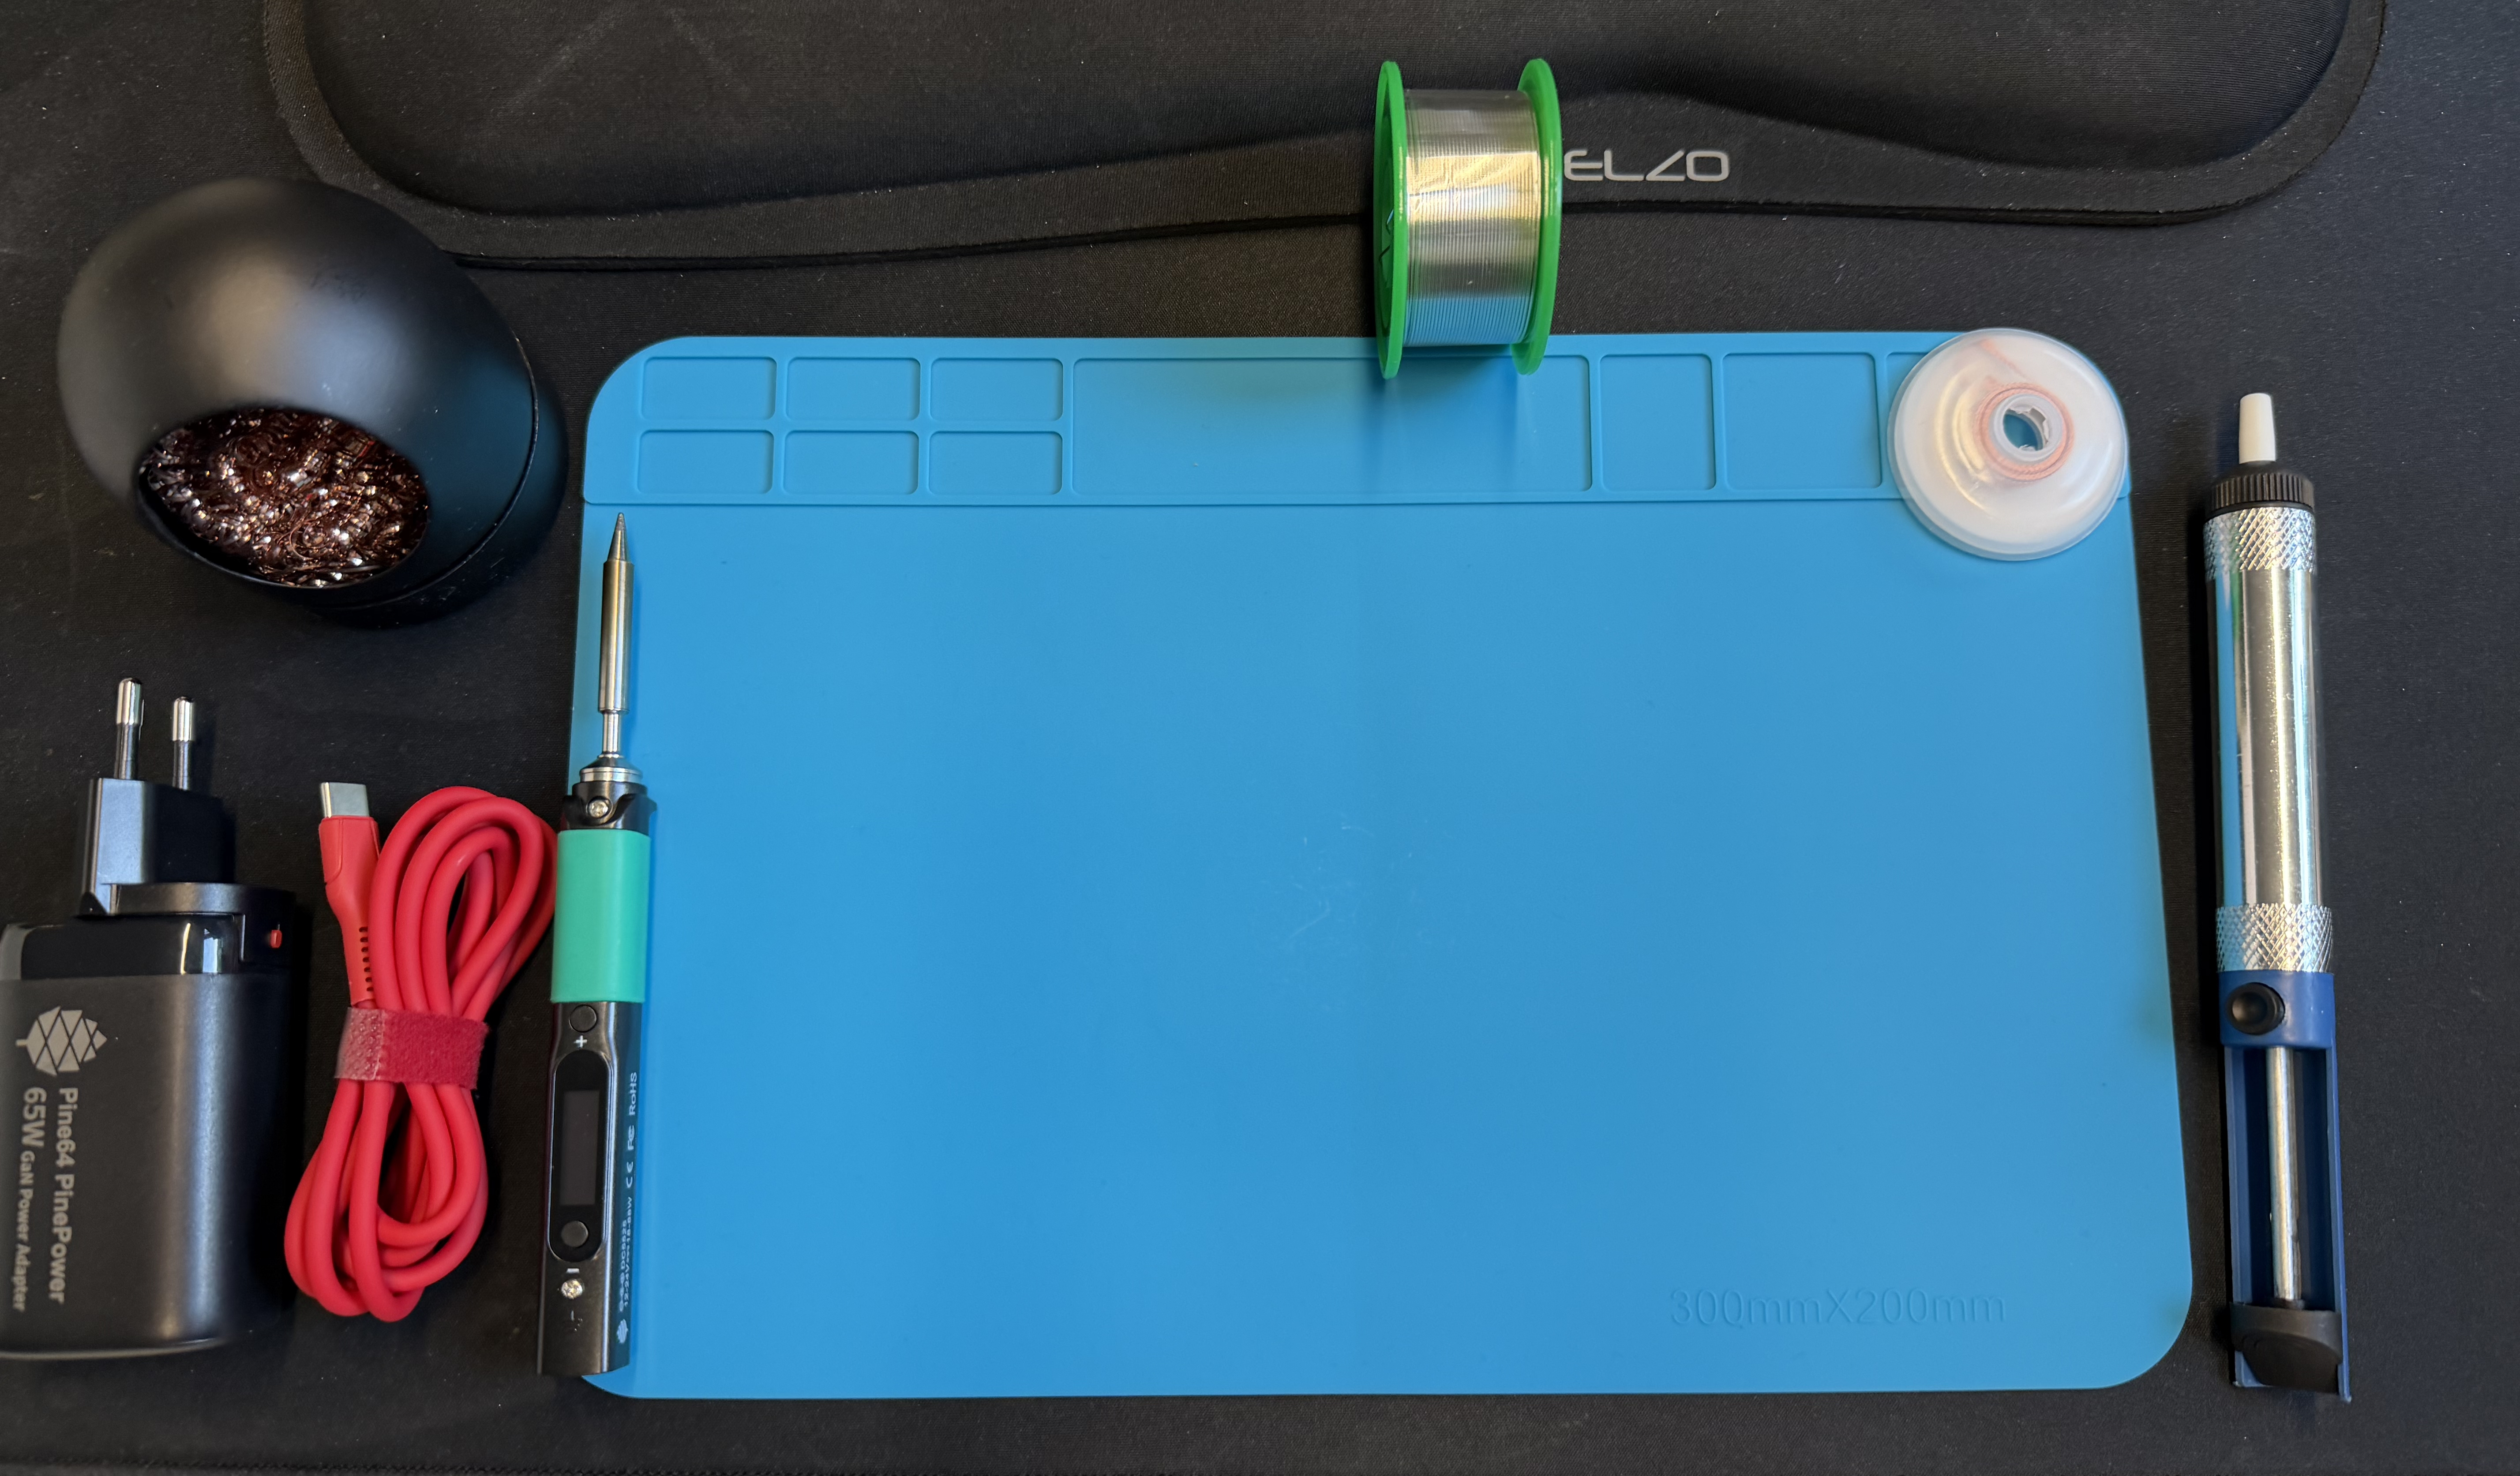
\includegraphics[width=\linewidth,keepaspectratio]{2.0.0.0_content/assets/bilder/setup.jpg}
    \end{column}
\end{columns}
\end{frame}

\begin{frame}{Wärmeführung}
\begin{columns}[T]
    \begin{column}{0.58\textwidth}
        \small
        \begin{itemize}\setlength{\itemsep}{3mm}
            \item Die Spitze berührt \textbf{gleichzeitig Pin und Pad}.
            \item Zuerst wird die \textbf{Verbindung erwärmt}, nicht sofort das Lot geschmolzen.
            \item So verteilt sich die Wärme besser und das Lot kann sauber fließen.
        \end{itemize}
        \normalsize
    \end{column}
    \begin{column}{0.42\textwidth}
        \centering
        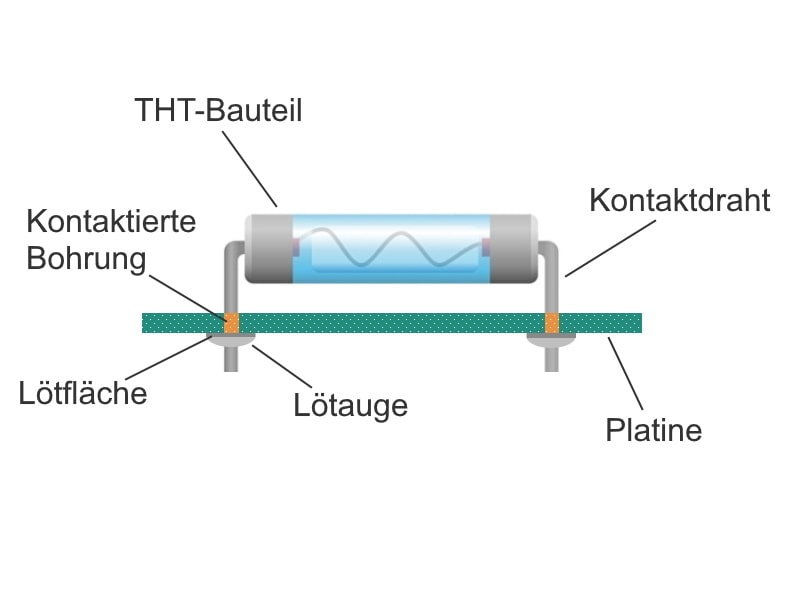
\includegraphics[width=\linewidth,keepaspectratio]{2.0.0.0_content/assets/bilder/tht_löten.jpg}
    \end{column}
\end{columns}
\end{frame}

\begin{frame}{Zinn zuführen}
\begin{columns}[T]
    \begin{column}{0.58\textwidth}
        \small
        \begin{itemize}\setlength{\itemsep}{3mm}
            \item Das \textbf{Lötzinn an die erhitzte Stelle} geben, nicht direkt an die Spitze.
            \item Dabei nutzt man die \textbf{Kapillarwirkung}, damit sich das Lot sauber verteilt.
            \item Meist gilt: \textbf{Weniger ist besser} als zu viel.
        \end{itemize}
        \normalsize
    \end{column}
    \begin{column}{0.42\textwidth}
        \centering
        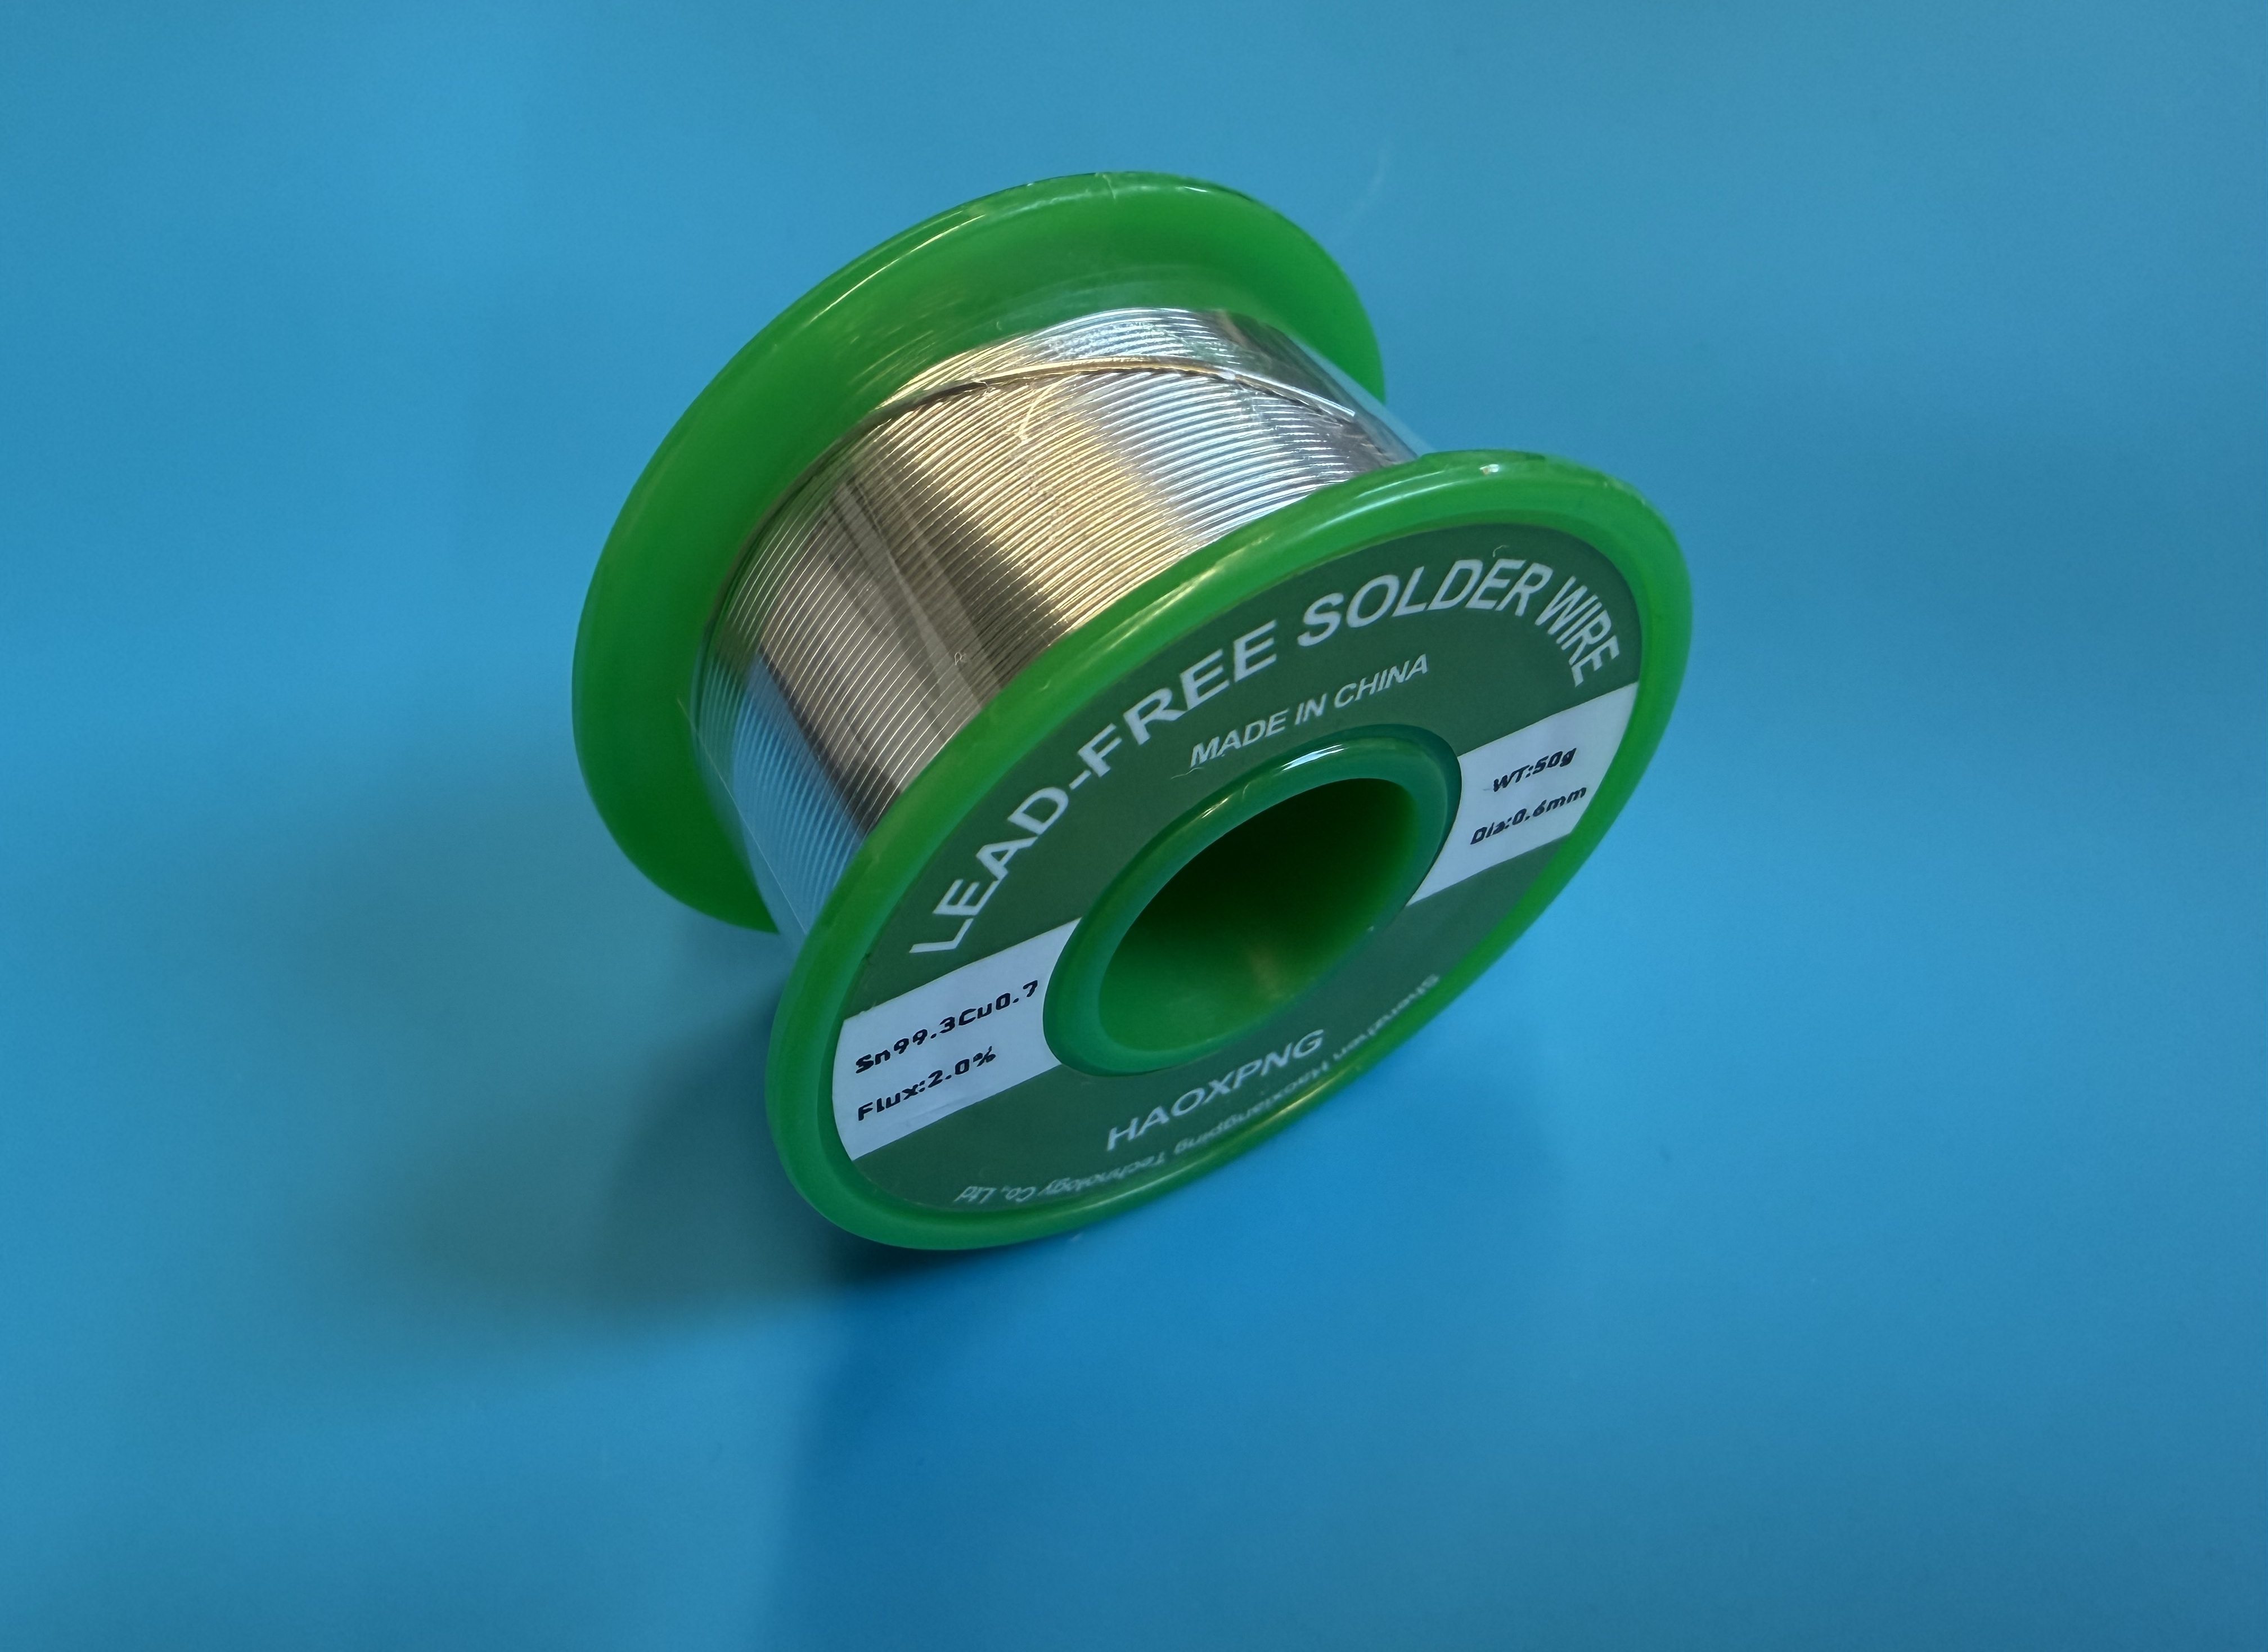
\includegraphics[width=\linewidth,keepaspectratio]{2.0.0.0_content/assets/bilder/lötzinn.jpg}
    \end{column}
\end{columns}
\end{frame}

\begin{frame}{Absetzen und Prüfen}
\begin{columns}[T]
    \begin{column}{0.58\textwidth}
        \small
        \begin{itemize}\setlength{\itemsep}{3mm}
            \item Zuerst das \textbf{Lot wegnehmen}, dann die \textbf{Lötspitze}.
            \item Die Lötstelle kurz \textbf{ruhig abkühlen lassen}.
            \item Danach folgt die \textbf{Sichtprüfung}: Form, Glanz und Sauberkeit kontrollieren.
        \end{itemize}
        \normalsize
    \end{column}
    \begin{column}{0.42\textwidth}
        \centering
        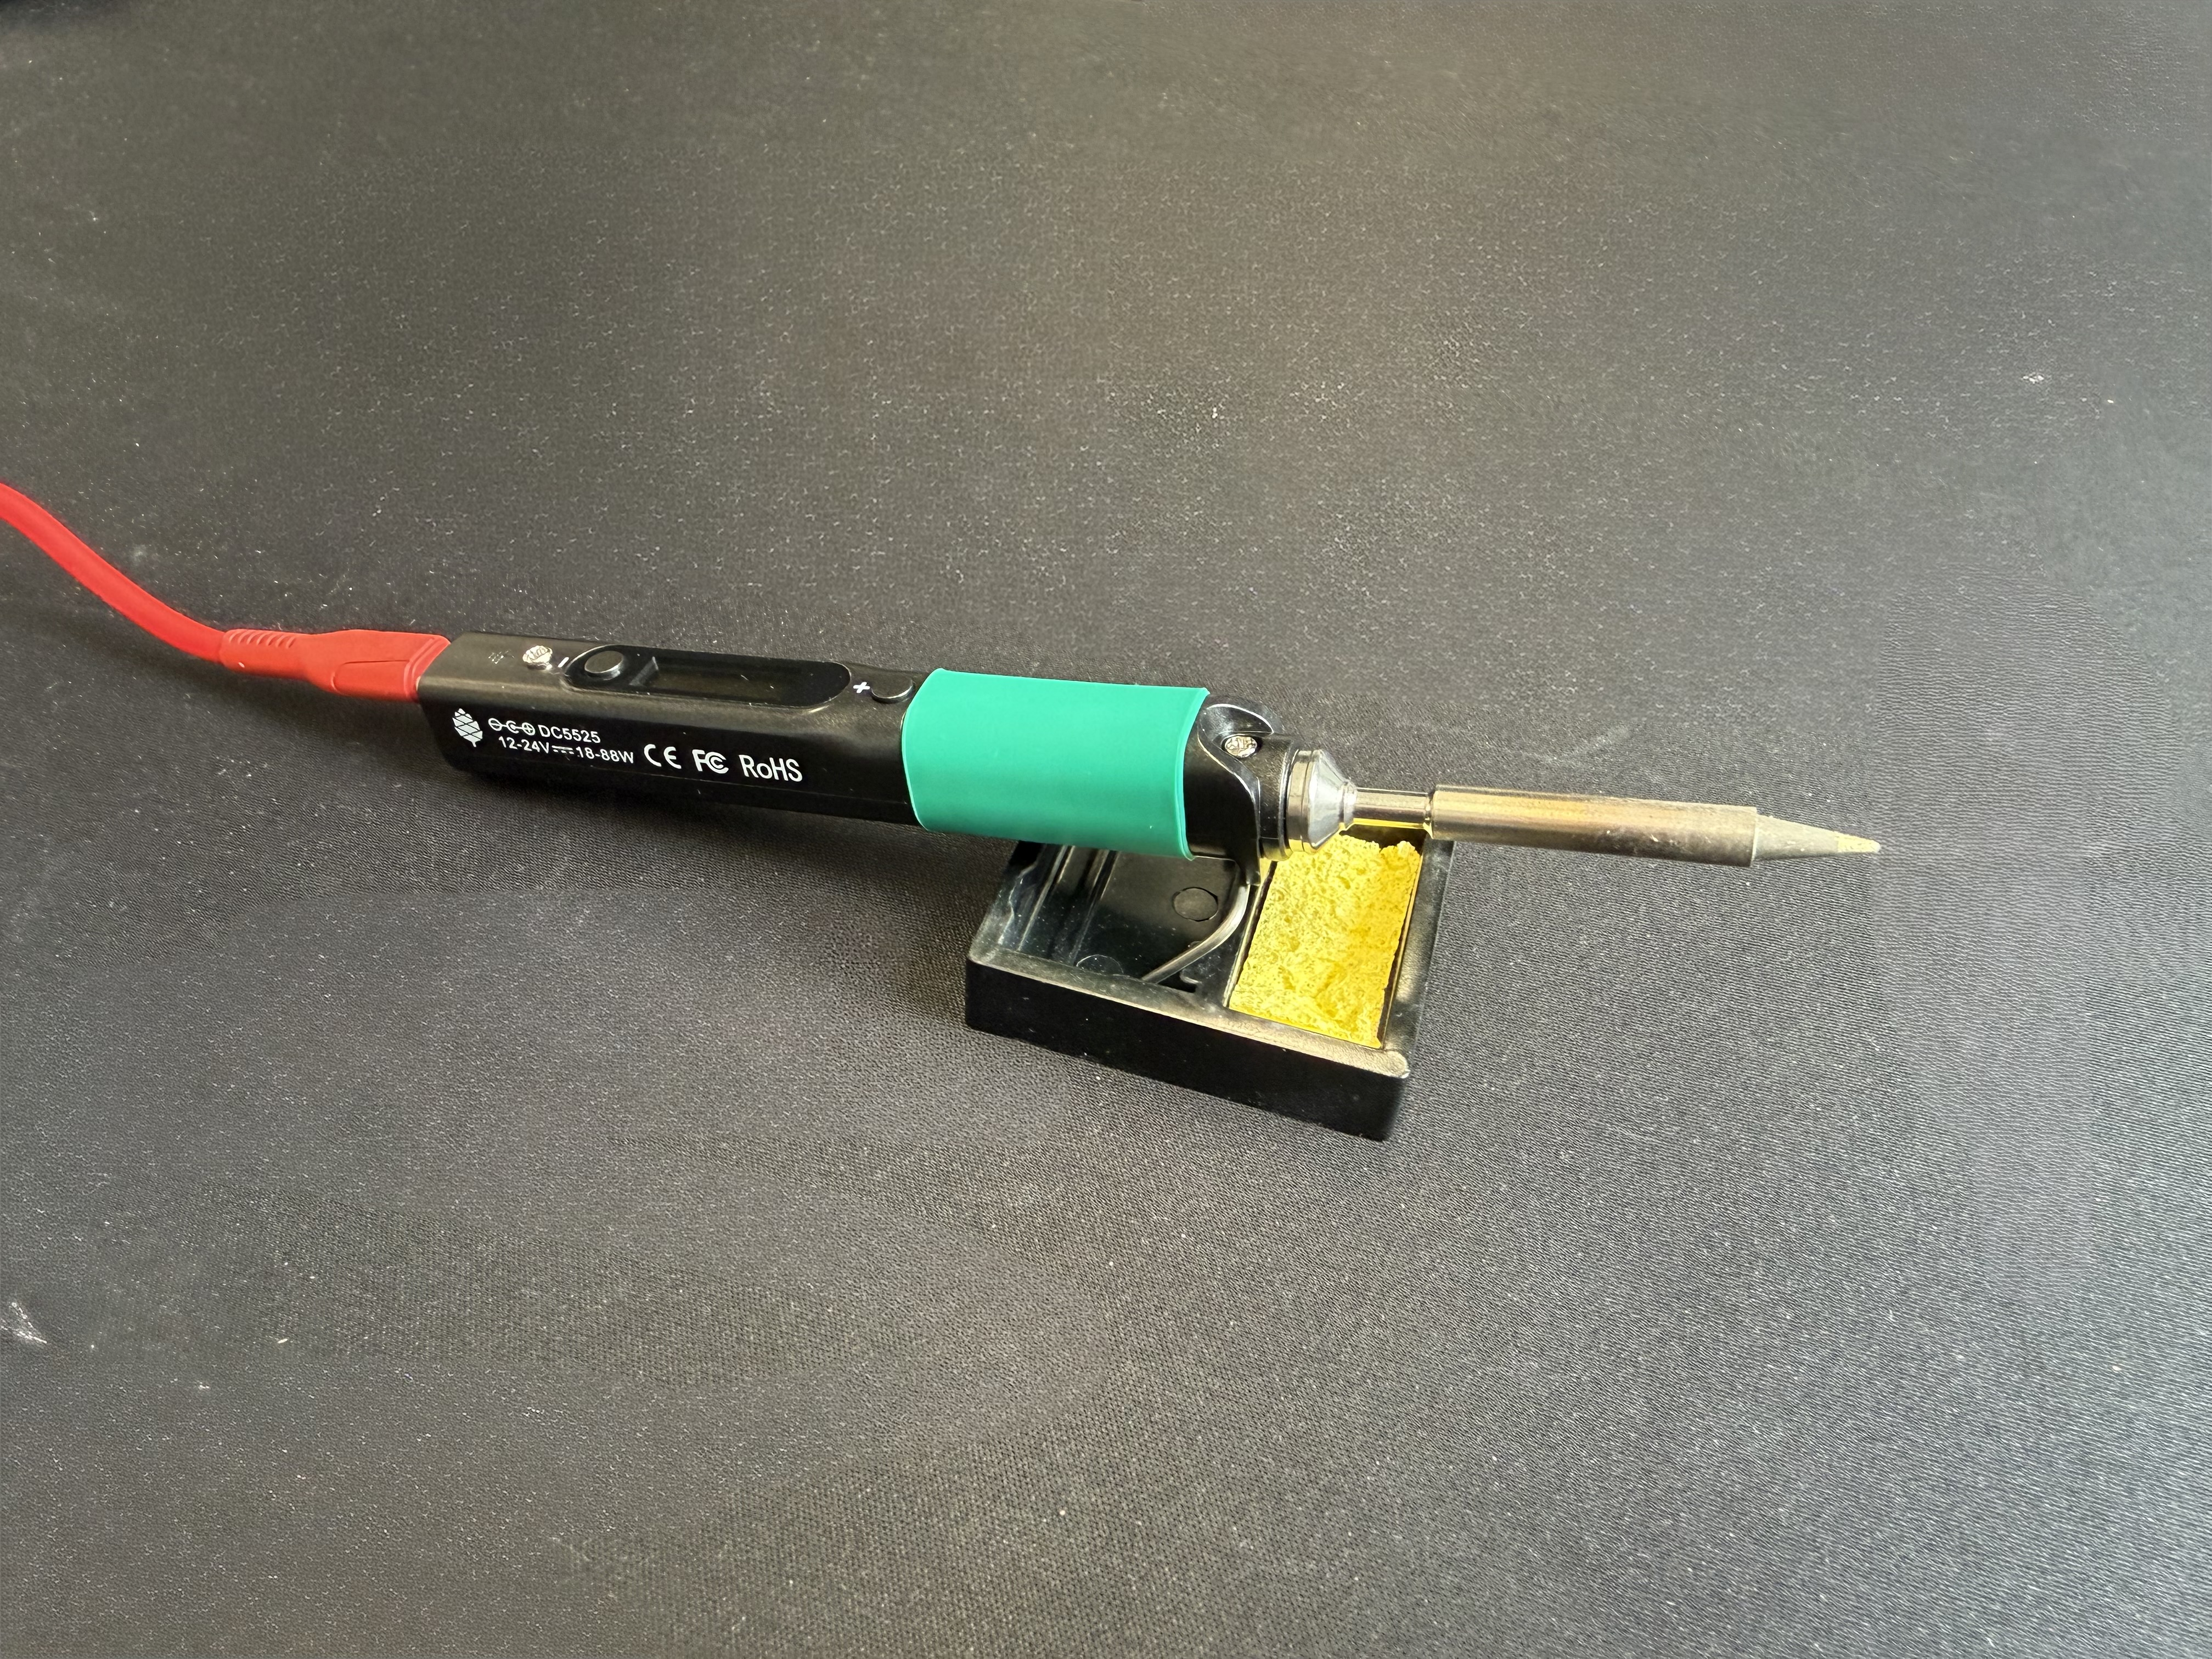
\includegraphics[width=\linewidth,keepaspectratio]{2.0.0.0_content/assets/bilder/lötkolben_abstellen.jpeg}
    \end{column}
\end{columns}
\end{frame}

\begin{frame}{Nacharbeit}
\begin{columns}[T]
    \begin{column}{0.58\textwidth}
        \small
        \begin{itemize}\setlength{\itemsep}{3mm}
            \item Überstehende Beinchen mit dem \textbf{Seitenschneider} kürzen.
            \item Während des Abkühlens die Lötstelle \textbf{nicht bewegen}.
            \item Wenn etwas nicht stimmt, lieber \textbf{noch einmal sauber neu aufbauen}.
        \end{itemize}
        \normalsize
    \end{column}
    \begin{column}{0.42\textwidth}
        \centering
        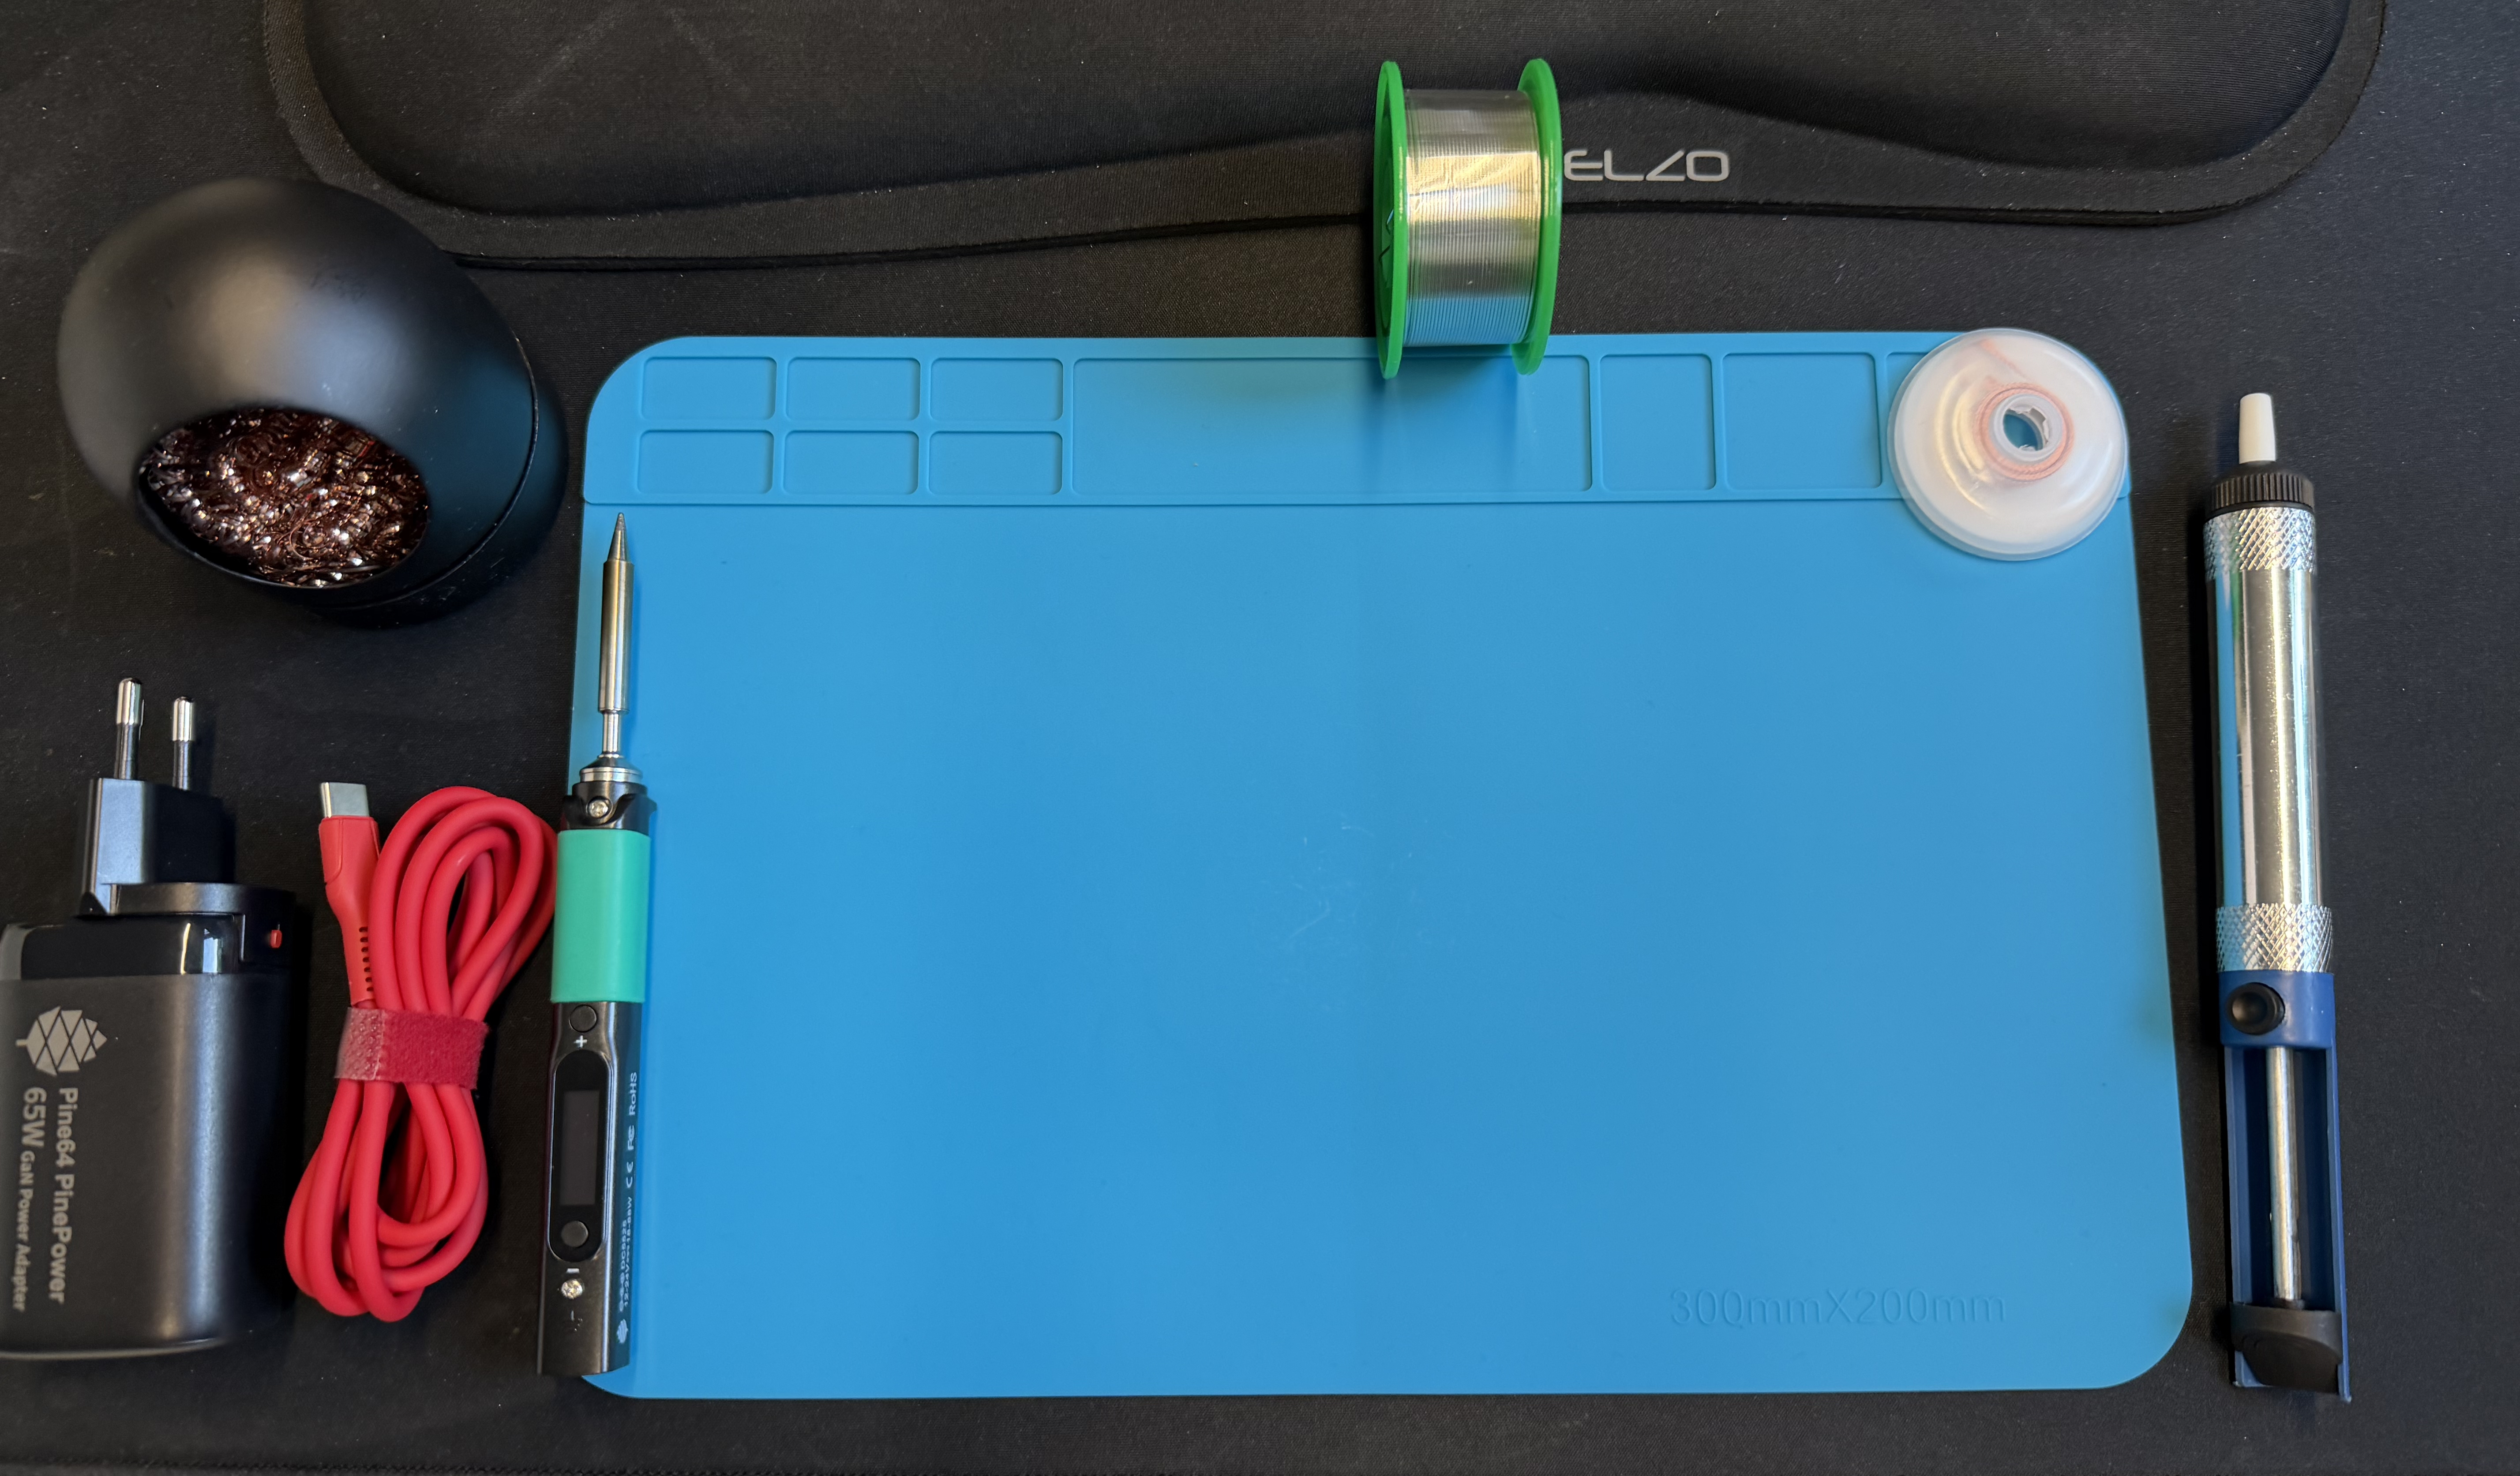
\includegraphics[width=\linewidth,keepaspectratio]{2.0.0.0_content/assets/bilder/setup.jpg}
    \end{column}
\end{columns}
\end{frame}

\begin{frame}{Temperatur und Zeit}
\begin{columns}[T]
    \begin{column}{0.58\textwidth}
        \small
        \begin{itemize}\setlength{\itemsep}{3mm}
            \item Nicht \textbf{zu kalt}, aber auch nicht \textbf{unnötig heiß} arbeiten.
            \item Ziel ist eine \textbf{kurze, saubere und kontrollierte} Erwärmung.
            \item Die \textbf{Boost-Funktion} nur kurz einsetzen, wenn mehr Wärme nötig ist.
        \end{itemize}
        \normalsize
    \end{column}
    \begin{column}{0.42\textwidth}
        \centering
        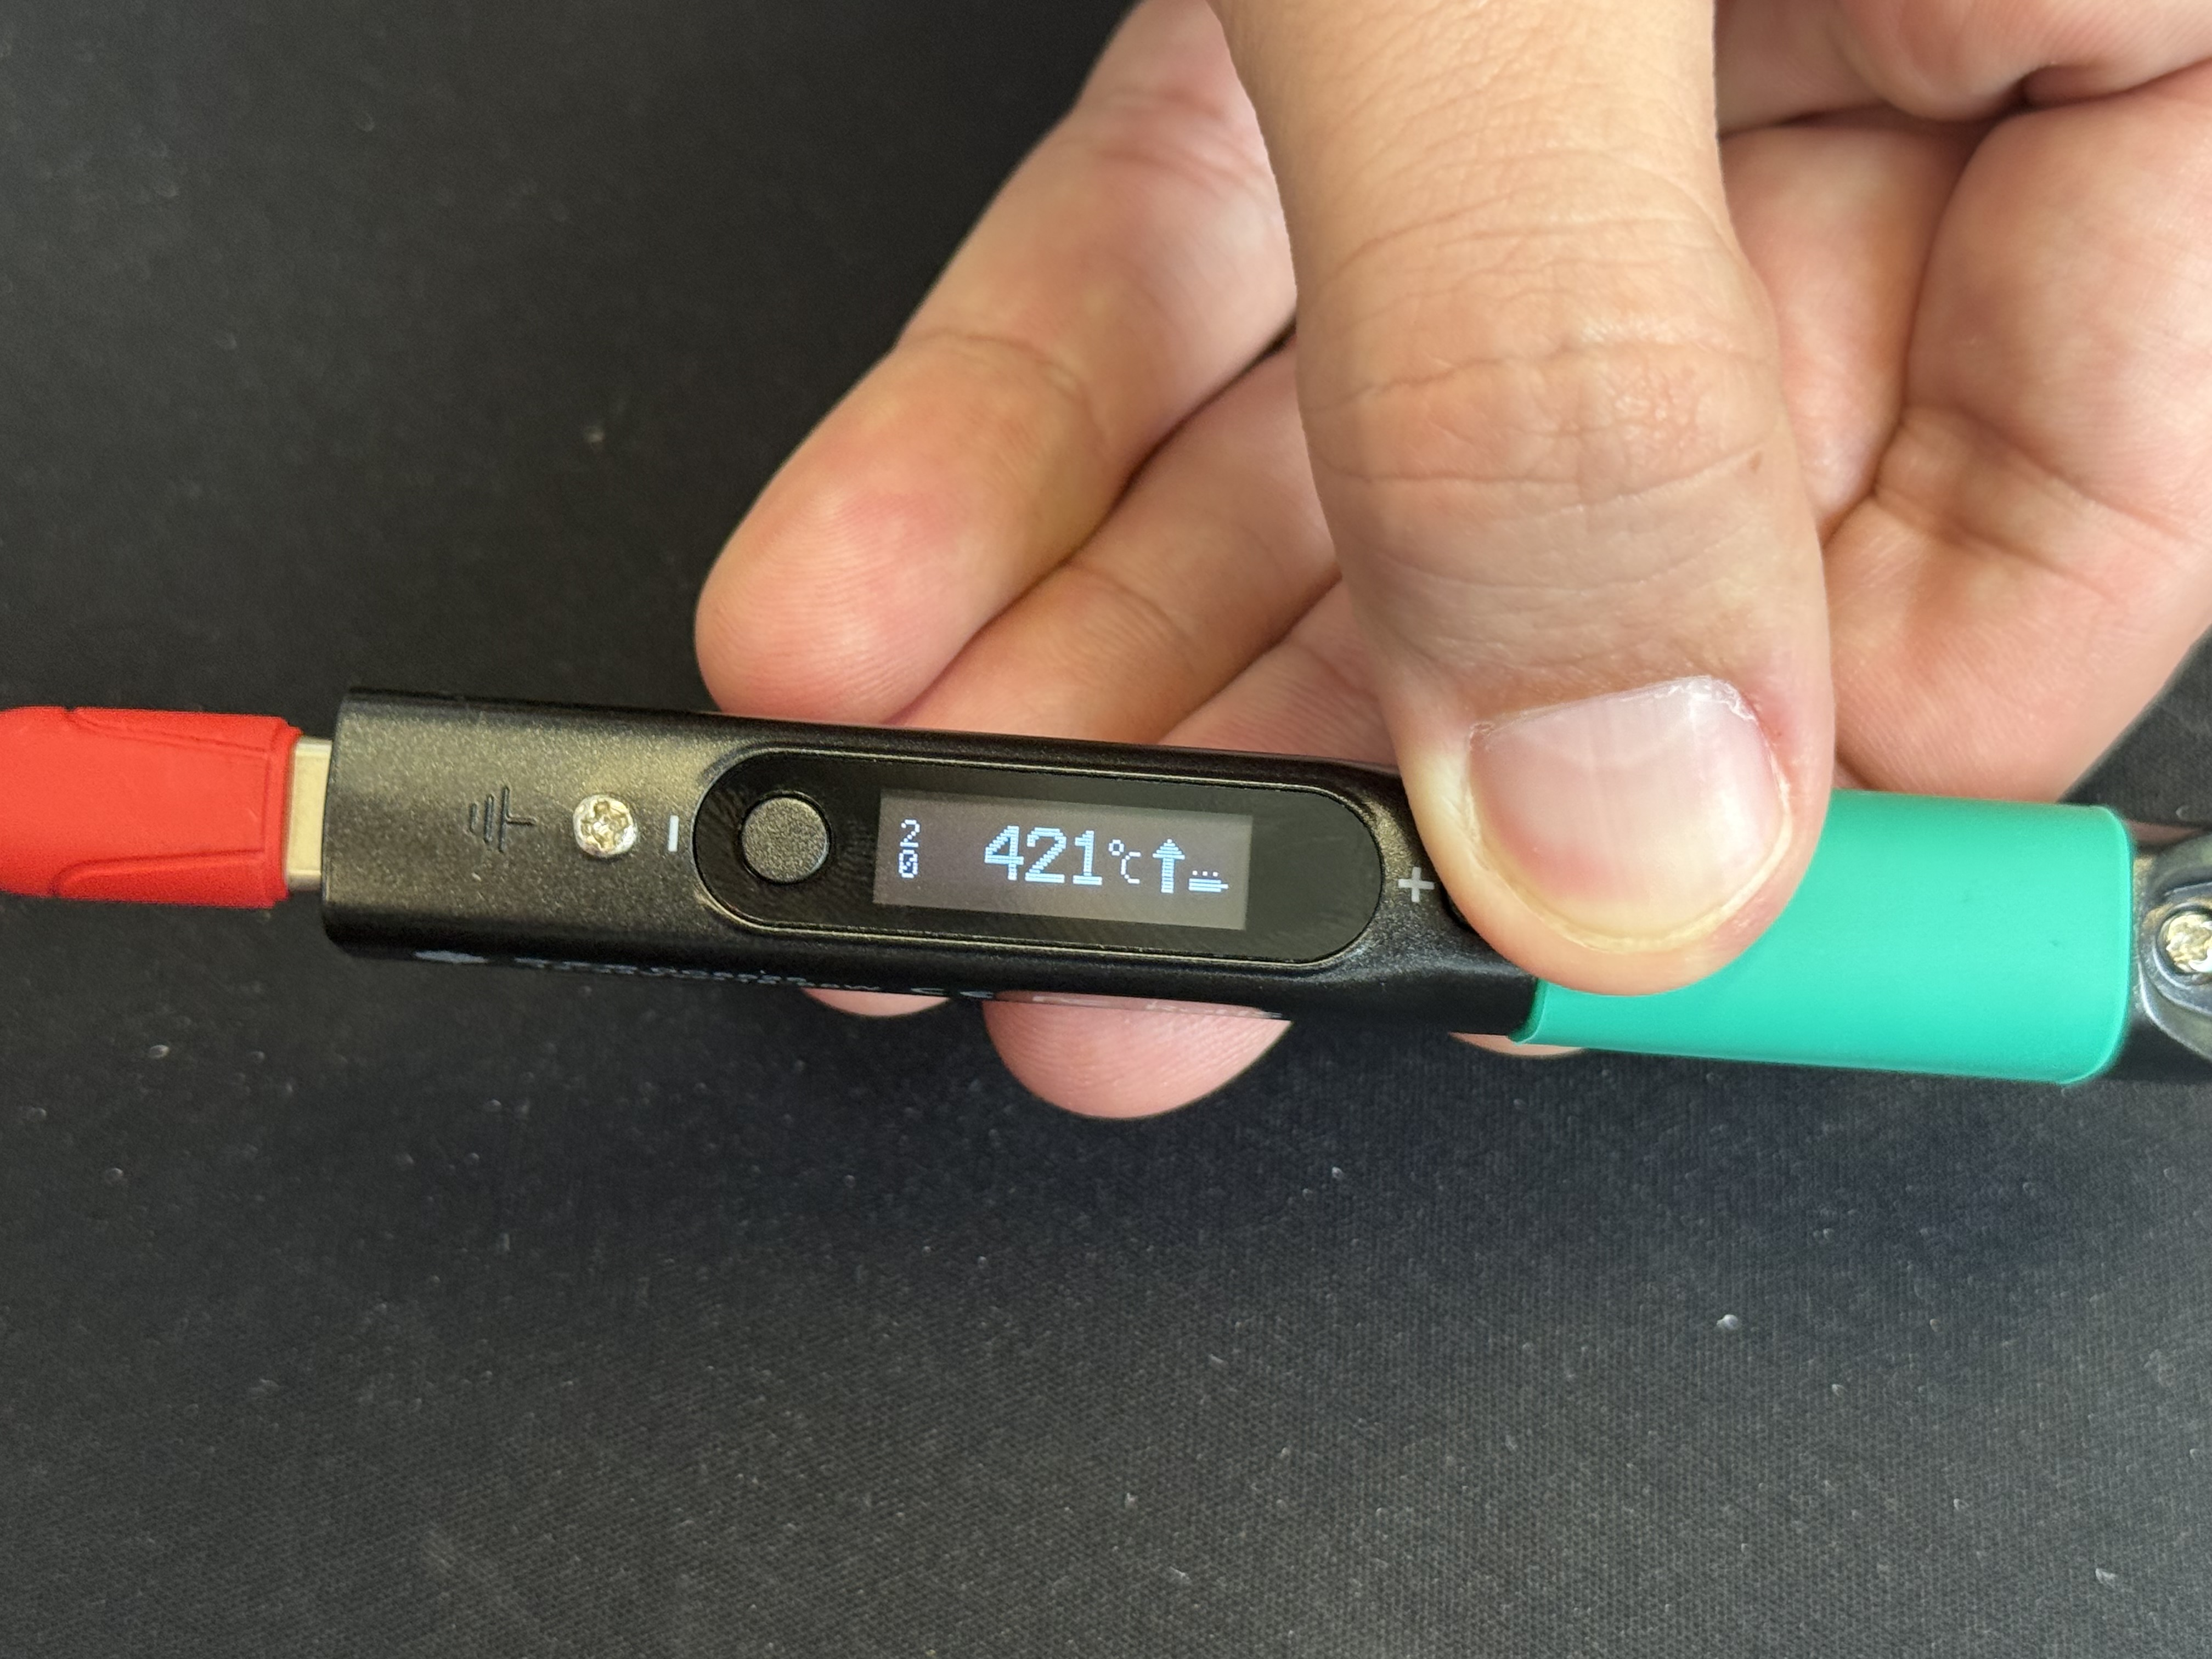
\includegraphics[width=\linewidth,keepaspectratio]{2.0.0.0_content/assets/bilder/lötkolben_Boost.jpeg}
    \end{column}
\end{columns}
\end{frame}

% Block 6: Häufige Fehler und Lösungen
\begin{frame}{Kalte Lötstelle}
\begin{columns}[T]
    \begin{column}{0.58\textwidth}
        \small
        \begin{itemize}\setlength{\itemsep}{3mm}
            \item Eine kalte Lötstelle wirkt oft \textbf{matt}, \textbf{körnig} oder instabil.
            \item Elektrisch kann der Kontakt schlecht sein, mechanisch wackelt die Verbindung.
            \item \textbf{Lösung:} erneut erwärmen und bei Bedarf \textbf{wenig Lot} sauber nachführen.
        \end{itemize}
        \normalsize
    \end{column}
    \begin{column}{0.42\textwidth}
        \centering
        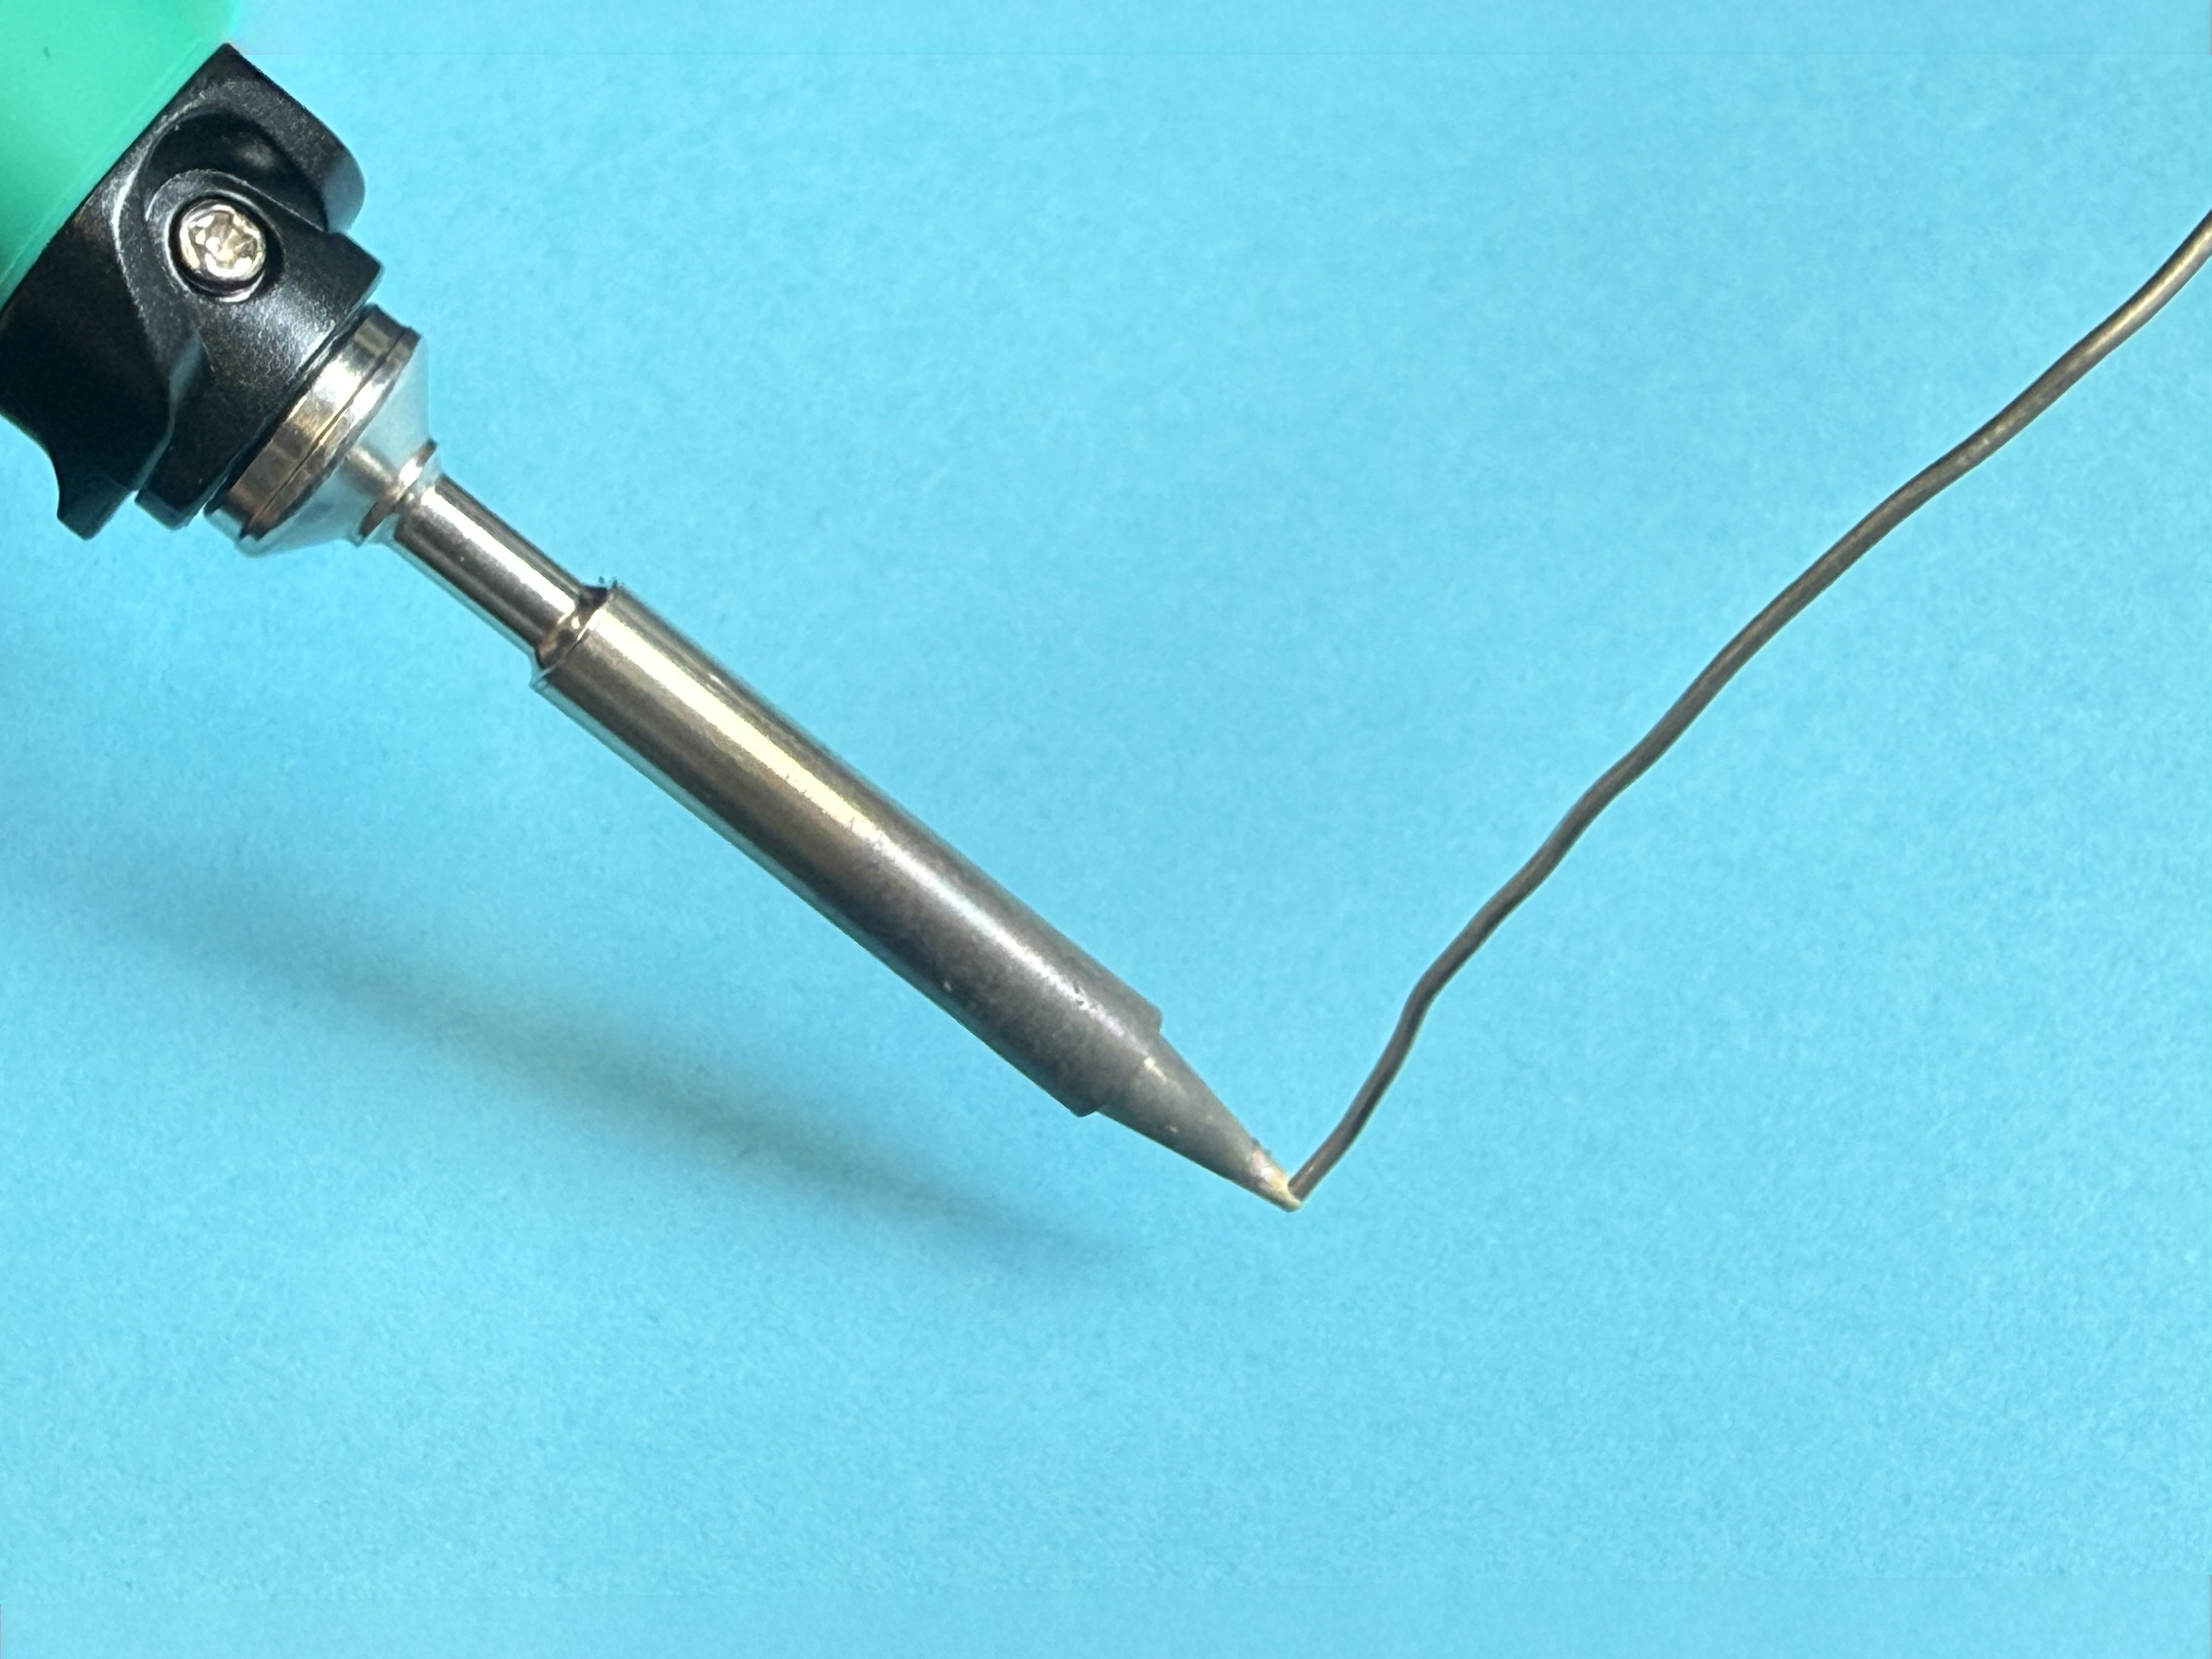
\includegraphics[width=\linewidth,keepaspectratio]{2.0.0.0_content/assets/bilder/zu_wenig_zinn.jpeg}
    \end{column}
\end{columns}
\end{frame}

\begin{frame}{Zu viel Zinn}
\begin{columns}[T]
    \begin{column}{0.58\textwidth}
        \small
        \begin{itemize}\setlength{\itemsep}{3mm}
            \item Zu viel Lot führt schnell zu \textbf{Kugelbildung} oder unsauberen Übergängen.
            \item Dadurch steigt das Risiko für \textbf{Brücken} und schlechte Nacharbeit.
            \item \textbf{Lösung:} Stelle erwärmen und überschüssiges Lot mit \textbf{Pumpe} oder \textbf{Litze} entfernen.
        \end{itemize}
        \normalsize
    \end{column}
    \begin{column}{0.42\textwidth}
        \centering
        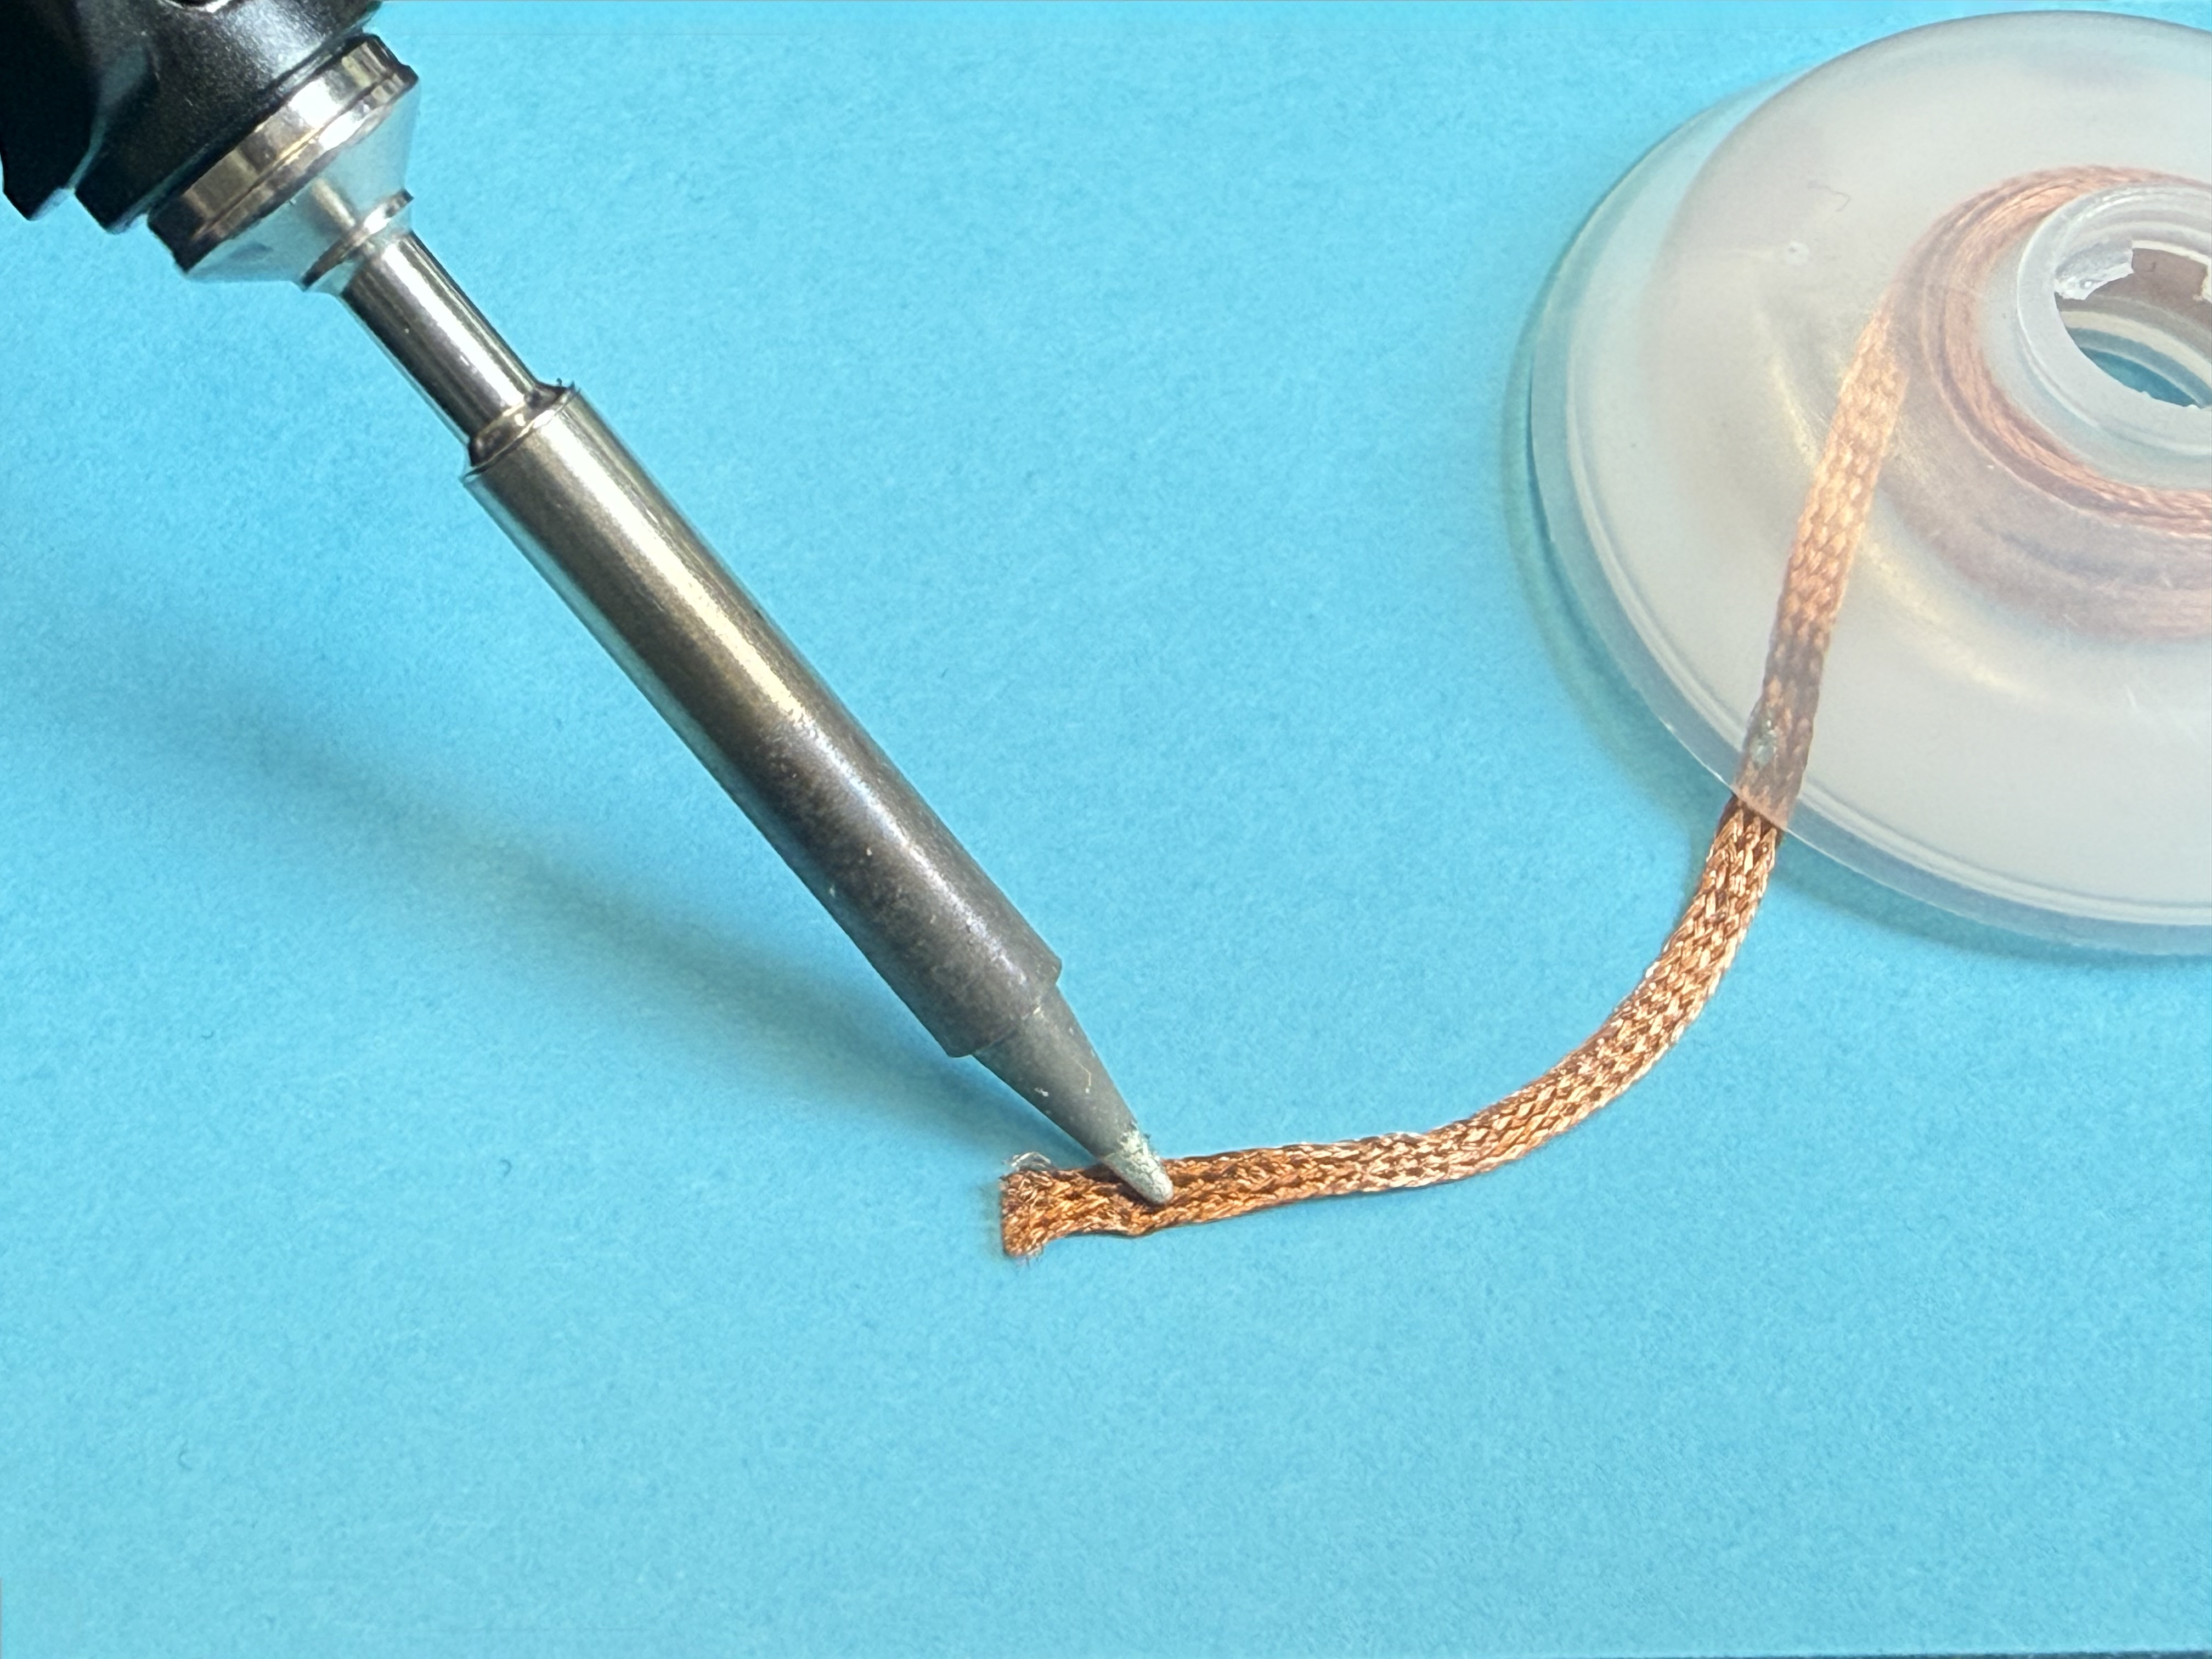
\includegraphics[width=\linewidth,keepaspectratio]{2.0.0.0_content/assets/bilder/zu_viel_zinn.jpeg}
    \end{column}
\end{columns}
\end{frame}

\begin{frame}{Zu wenig Zinn}
\begin{columns}[T]
    \begin{column}{0.58\textwidth}
        \small
        \begin{itemize}\setlength{\itemsep}{3mm}
            \item Ist zu wenig Lot vorhanden, wird das Pad oft \textbf{nicht vollständig benetzt}.
            \item Die Verbindung ist dann \textbf{schwach} oder unzuverlässig.
            \item \textbf{Lösung:} Stelle erneut erwärmen und \textbf{kontrolliert wenig Lot} nachführen.
        \end{itemize}
        \normalsize
    \end{column}
    \begin{column}{0.42\textwidth}
        \centering
        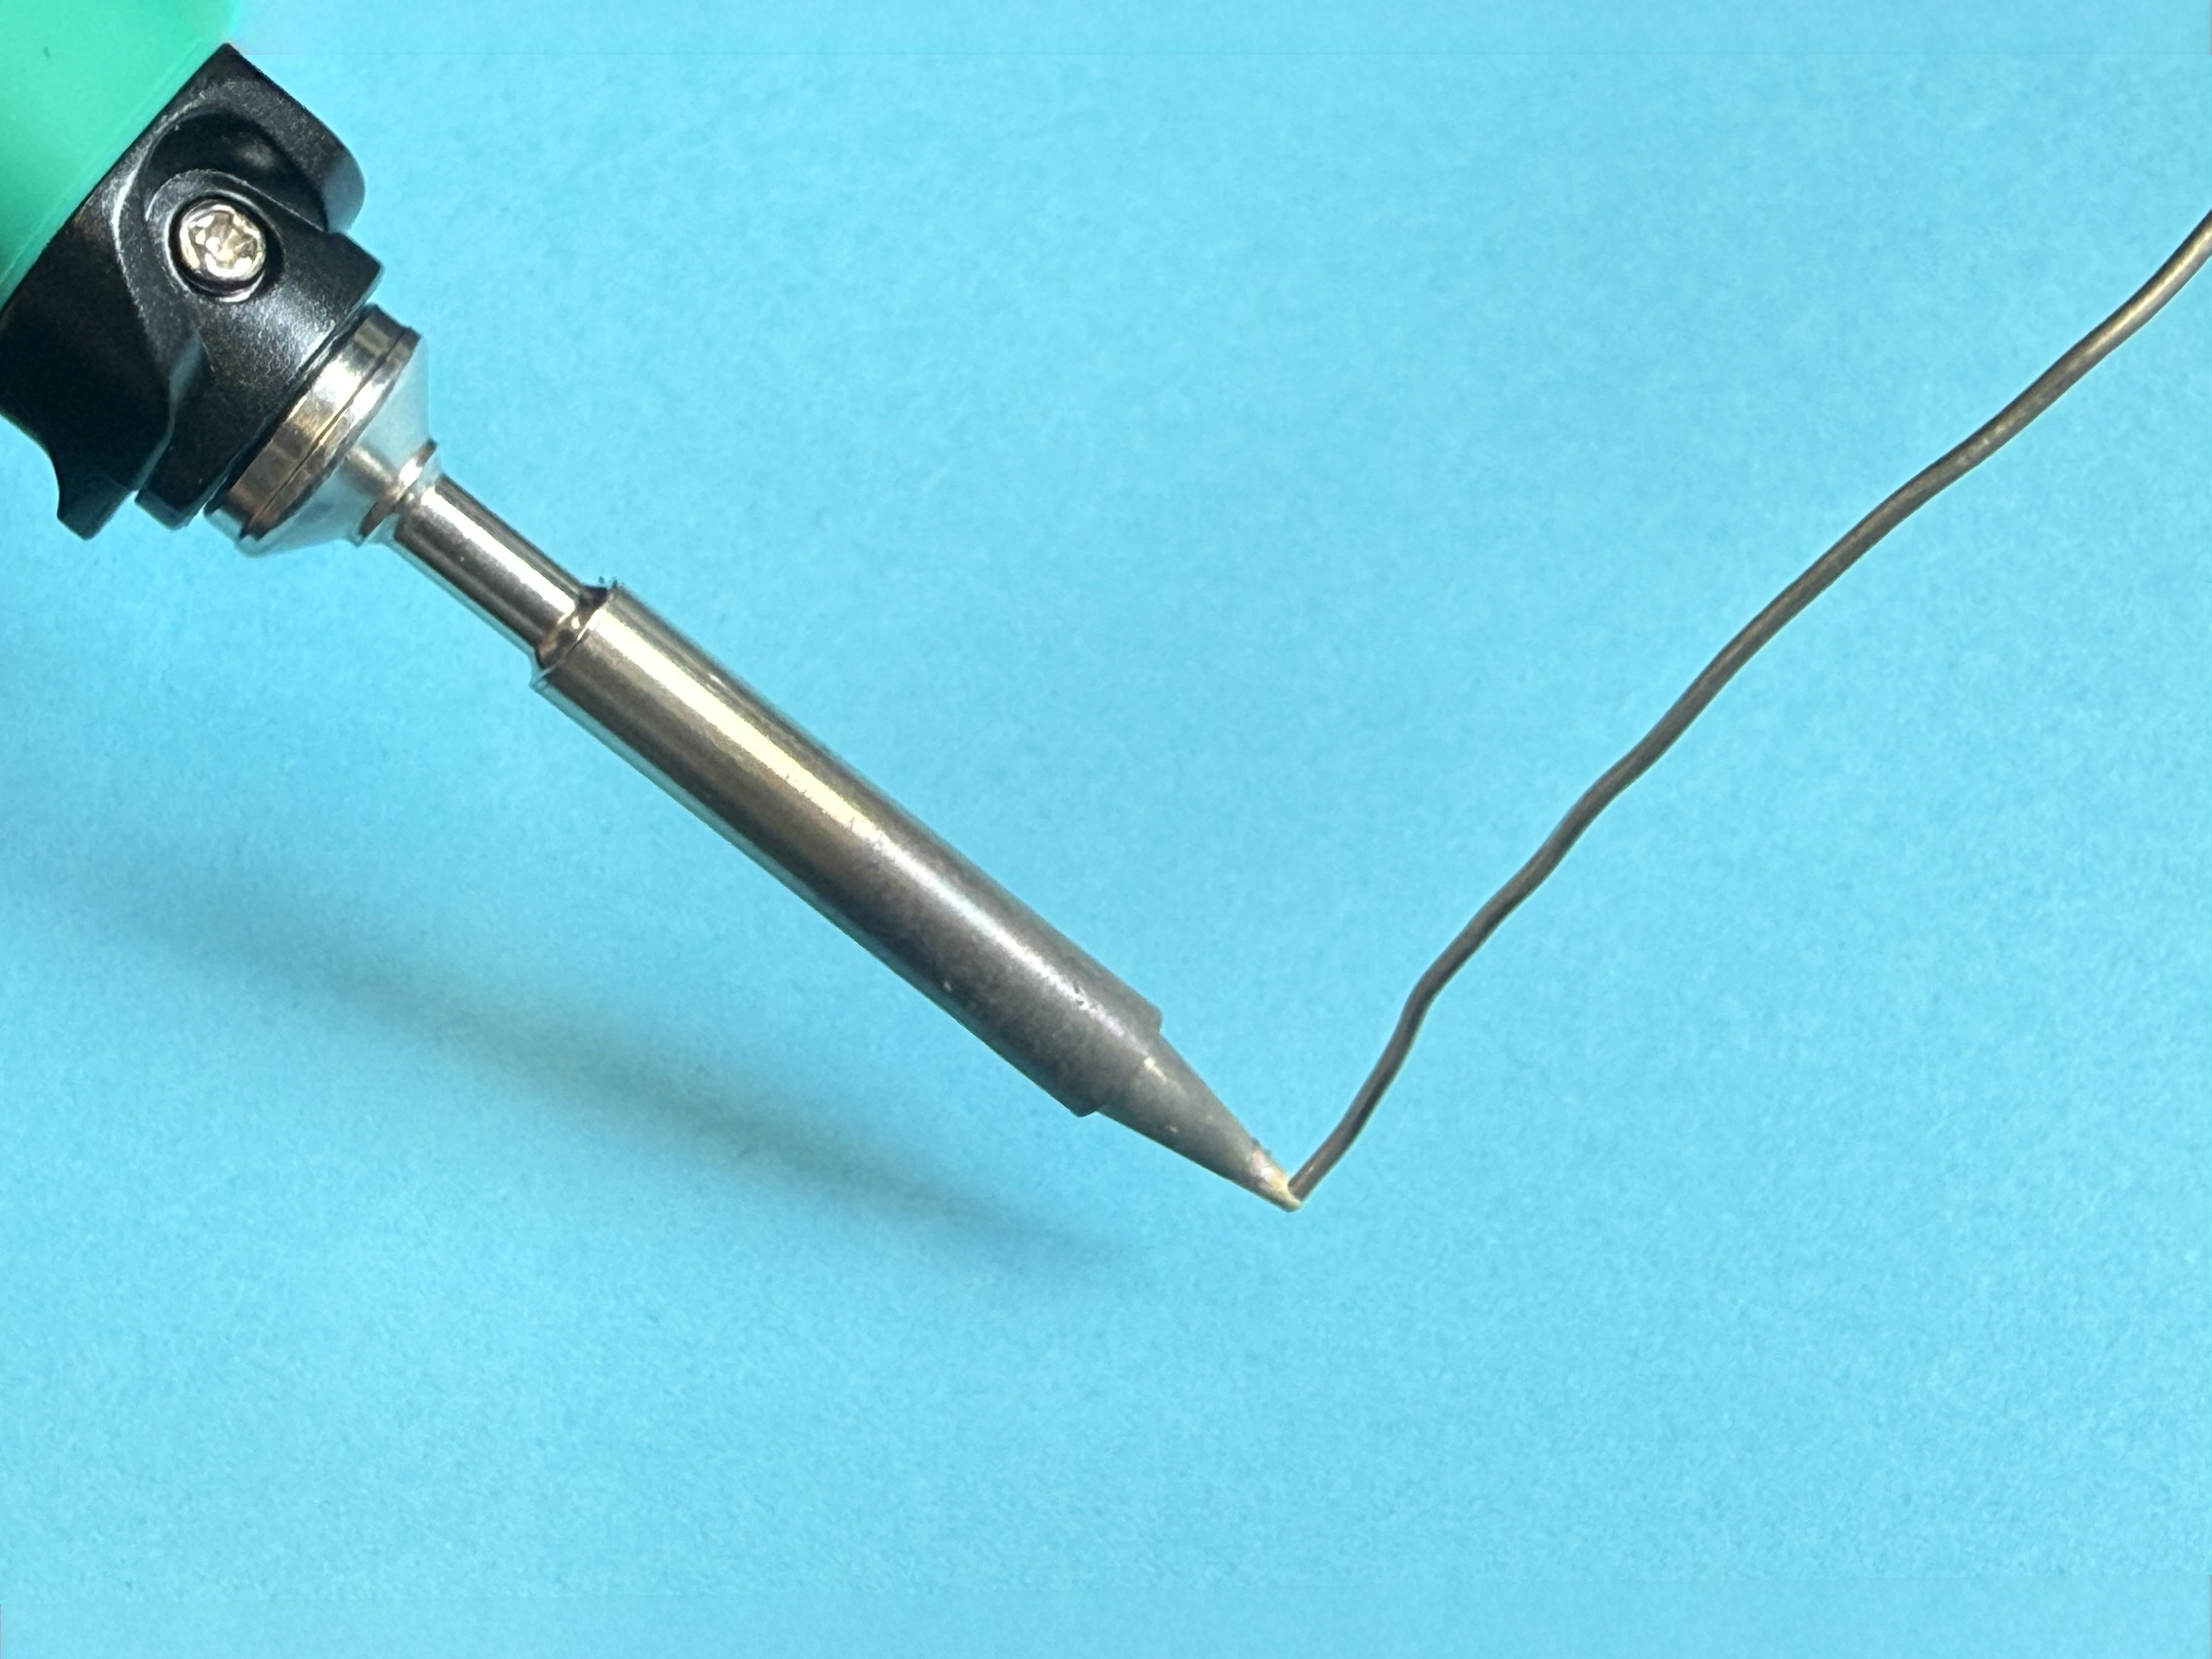
\includegraphics[width=\linewidth,keepaspectratio]{2.0.0.0_content/assets/bilder/zu_wenig_zinn.jpeg}
    \end{column}
\end{columns}
\end{frame}

\begin{frame}{Lötbrücke}
\begin{columns}[T]
    \begin{column}{0.58\textwidth}
        \small
        \begin{itemize}\setlength{\itemsep}{3mm}
            \item Eine Lötbrücke verbindet zwei Pads \textbf{ungewollt} miteinander.
            \item Das kann zu \textbf{Kurzschlüssen} oder Fehlfunktionen führen.
            \item \textbf{Lösung:} Litze verwenden und das überschüssige Lot \textbf{sauber abheben}.
        \end{itemize}
        \normalsize
    \end{column}
    \begin{column}{0.42\textwidth}
        \centering
        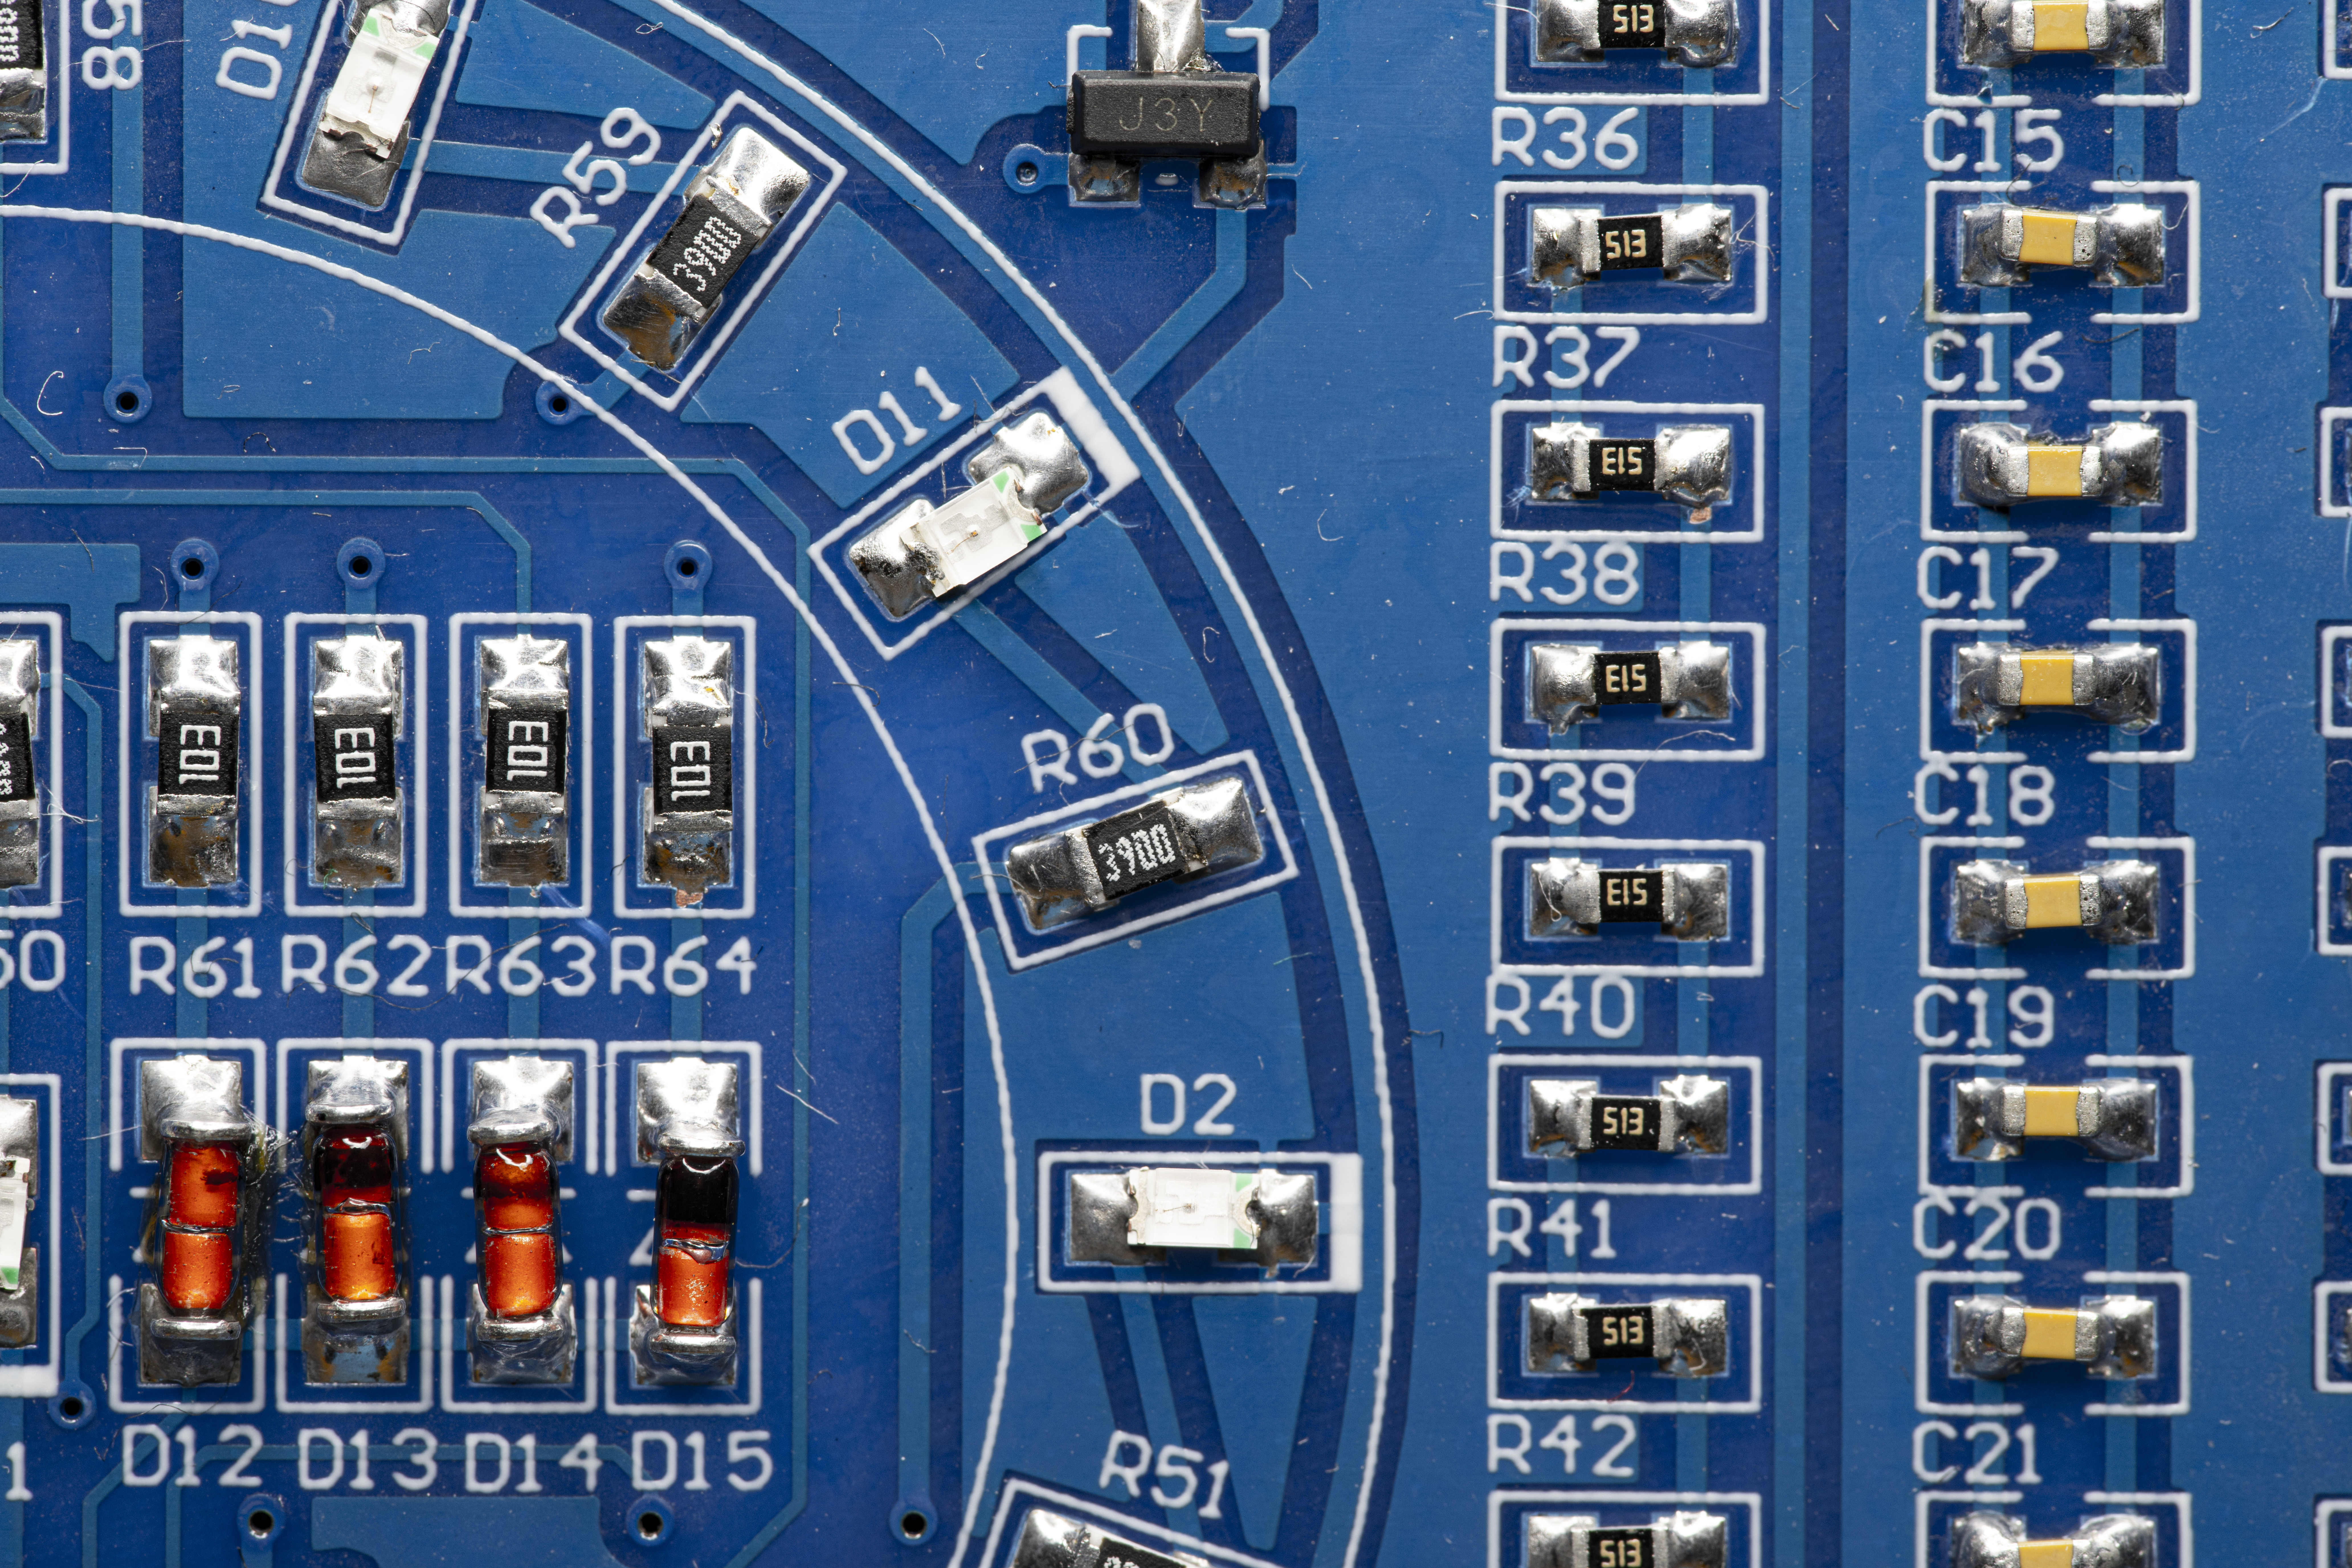
\includegraphics[width=\linewidth,keepaspectratio]{2.0.0.0_content/assets/bilder/smd_löten.jpg}
    \end{column}
\end{columns}
\end{frame}

\begin{frame}{Überhitzung}
\begin{columns}[T]
    \begin{column}{0.58\textwidth}
        \small
        \begin{itemize}\setlength{\itemsep}{3mm}
            \item Zu langes Erhitzen kann \textbf{Pads}, \textbf[Bauteile]{} oder Leiterbahnen schädigen.
            \item Typische Zeichen sind \textbf{Verfärbungen}, gelöste Pads oder gestresste Bauteile.
            \item \textbf{Lösung:} kürzer arbeiten, Pausen machen und die Temperatur passend wählen.
        \end{itemize}
        \normalsize
    \end{column}
    \begin{column}{0.42\textwidth}
        \centering
        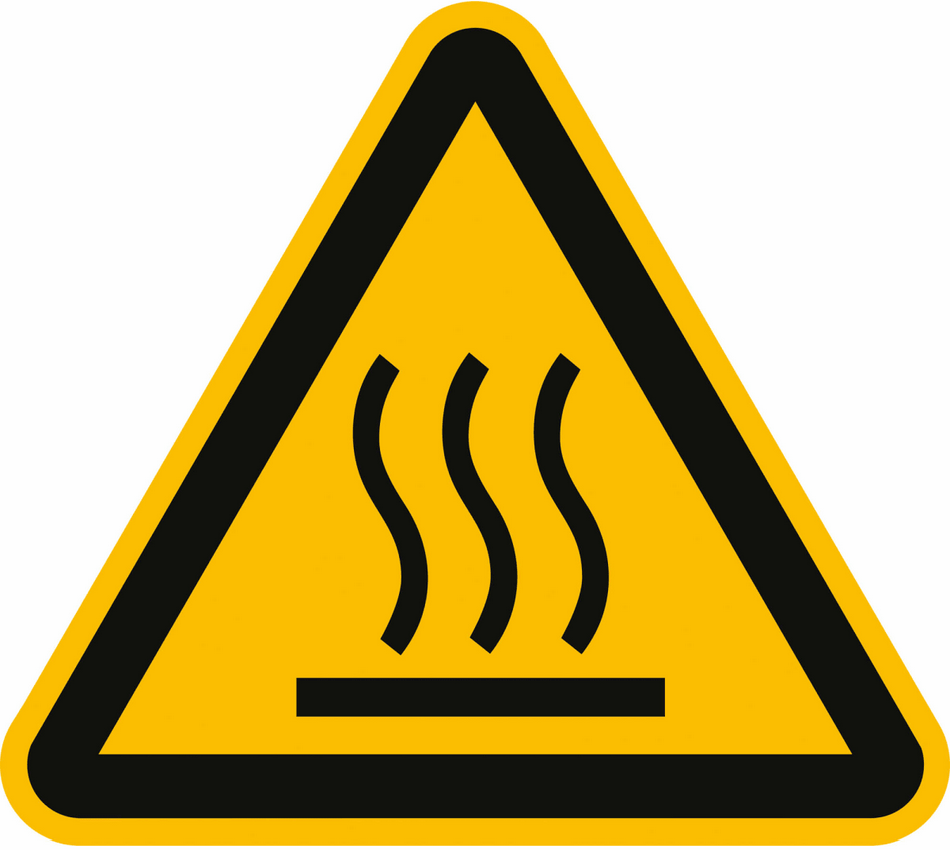
\includegraphics[width=\linewidth,keepaspectratio]{2.0.0.0_content/assets/bilder/Warnzeichen.png}
    \end{column}
\end{columns}
\end{frame}

\begin{frame}{Bauteil schief}
\begin{columns}[T]
    \begin{column}{0.58\textwidth}
        \small
        \begin{itemize}\setlength{\itemsep}{3mm}
            \item Sitzt ein Bauteil schief, wirkt die Verbindung \textbf{unsauber} und oft auch \textbf{mechanisch schlechter}.
            \item Gerade bei Steckleisten, Displays oder größeren Bauteilen fällt das schnell auf.
            \item \textbf{Lösung:} Lötstelle kurz verflüssigen, Bauteil \textbf{neu ausrichten} und ruhig abkühlen lassen.
        \end{itemize}
        \normalsize
    \end{column}
    \begin{column}{0.42\textwidth}
        \centering
        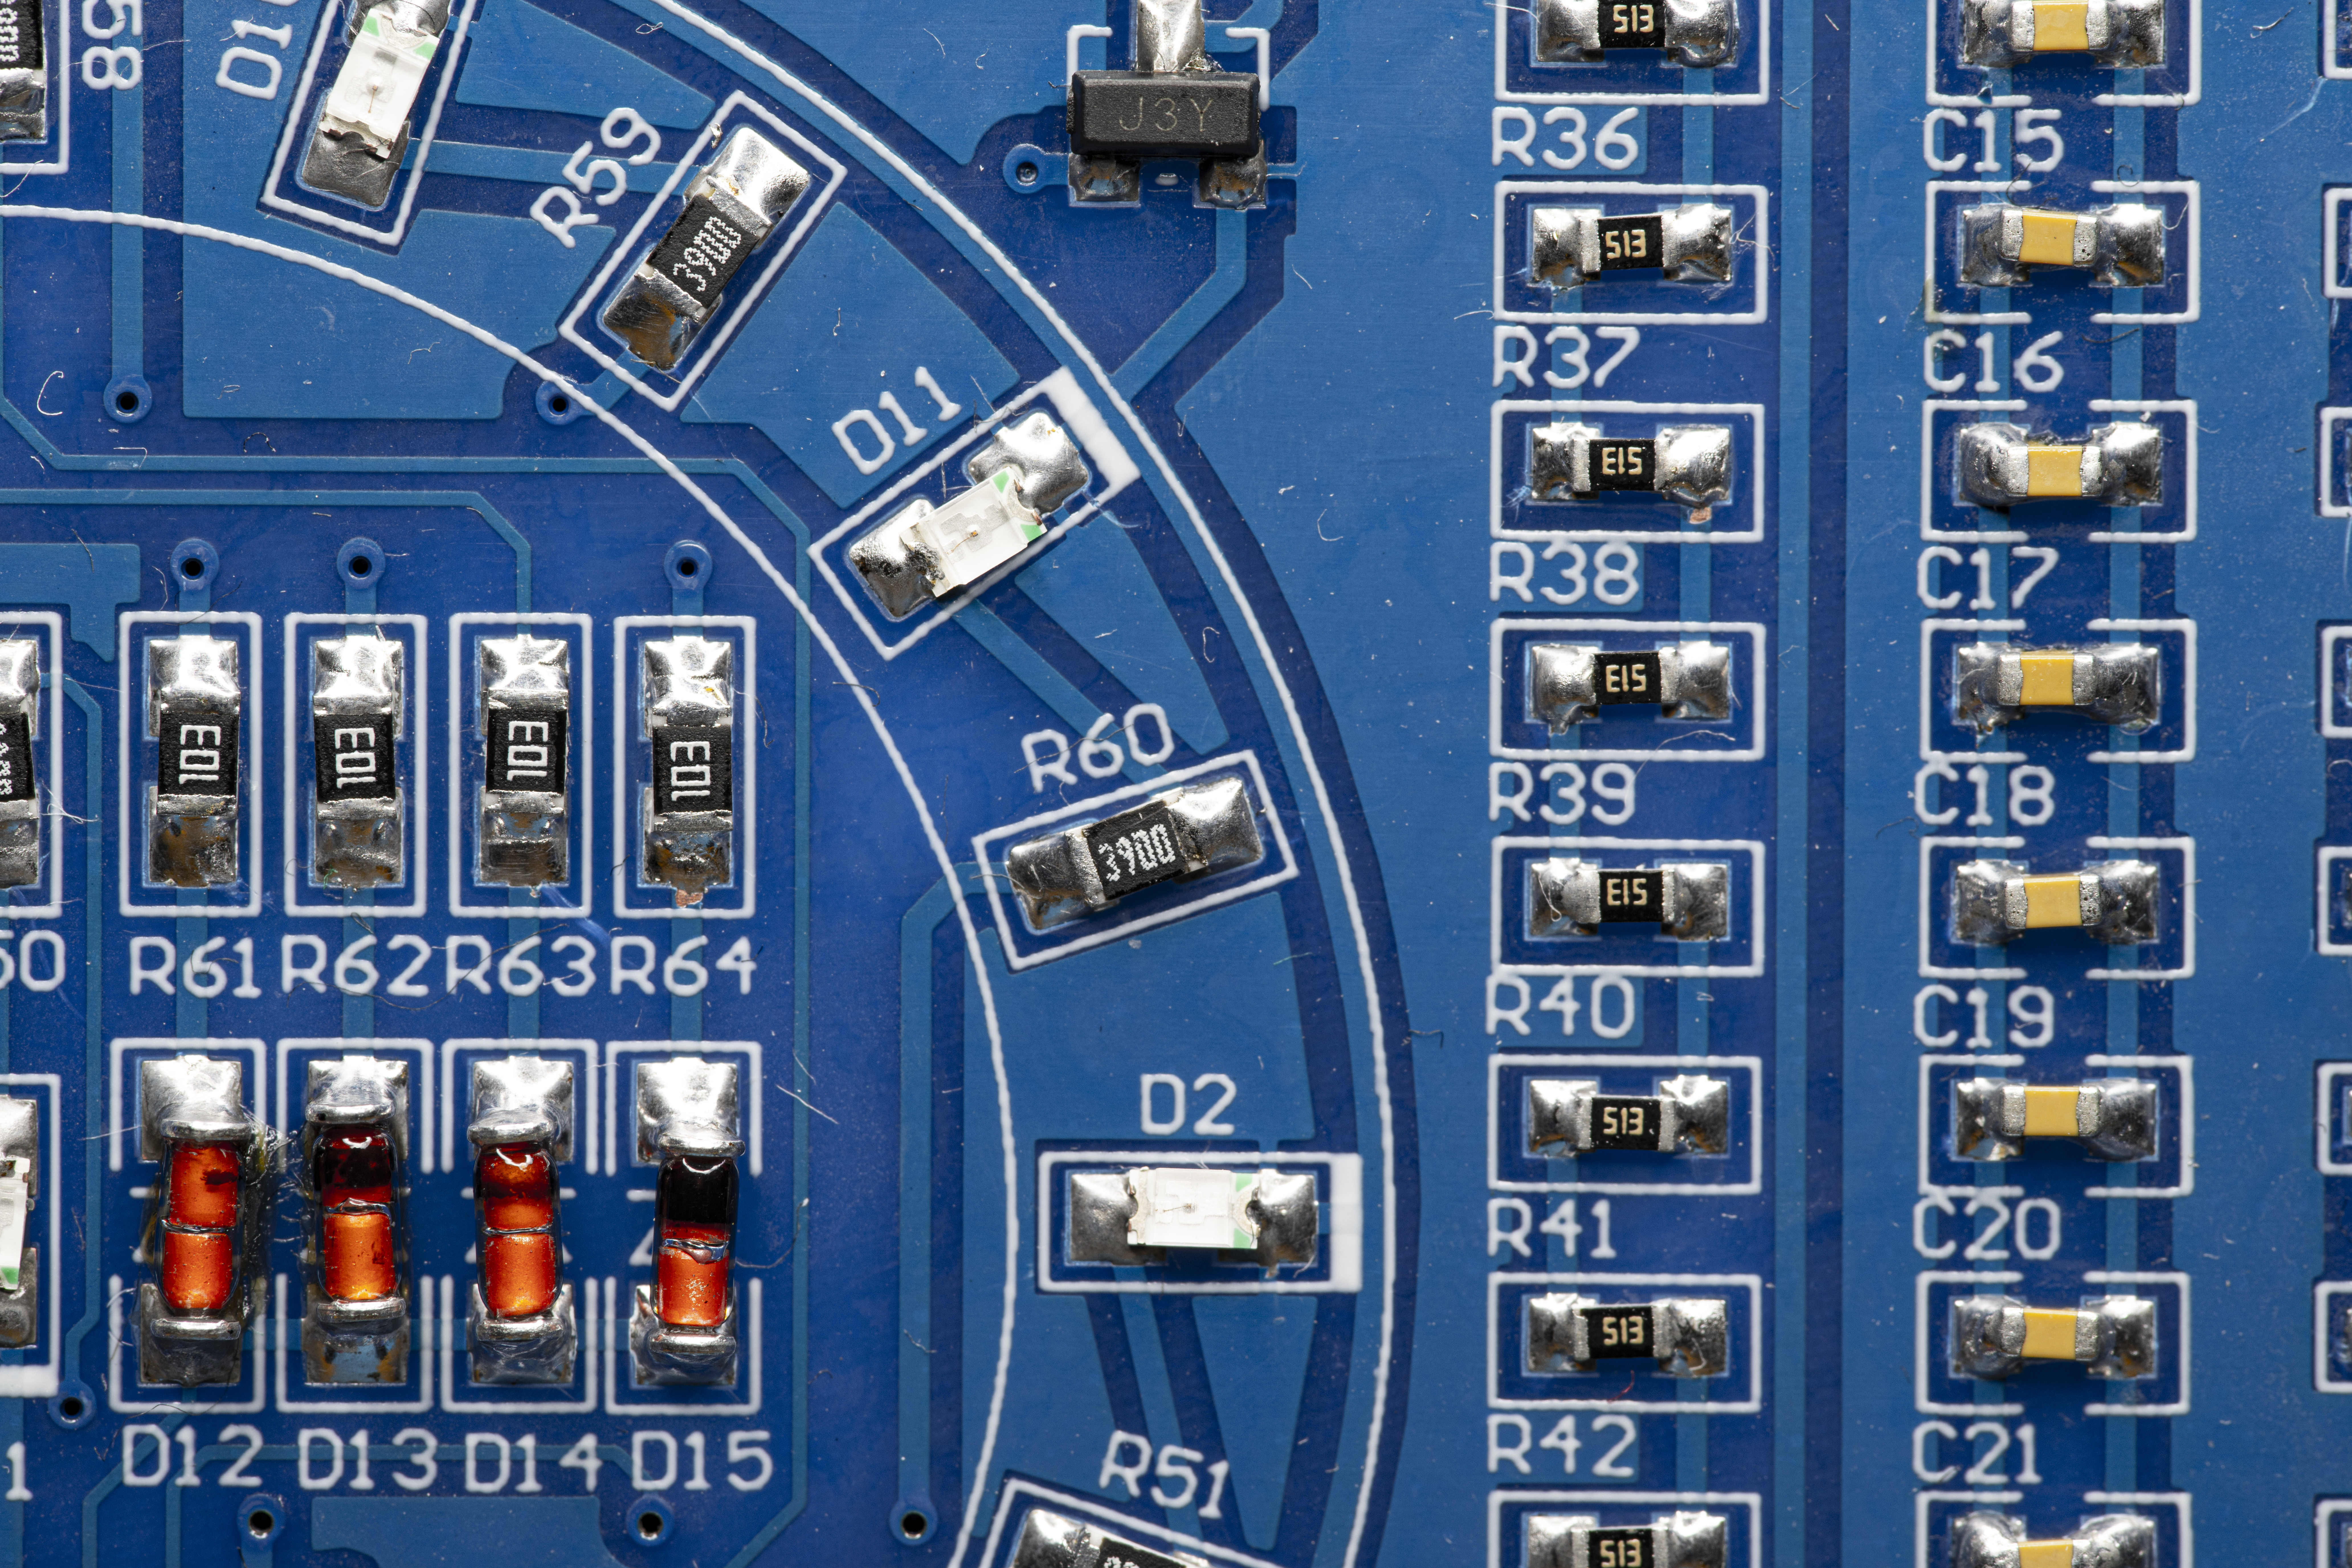
\includegraphics[width=\linewidth,keepaspectratio]{2.0.0.0_content/assets/bilder/smd_löten.jpg}
    \end{column}
\end{columns}
\end{frame}

% Block 7: Kontrolle und Praxis
\begin{frame}{Inspektion}
\begin{columns}[T]
    \begin{column}{0.58\textwidth}
        \small
        \begin{itemize}\setlength{\itemsep}{3mm}
            \item Zur Kontrolle helfen \textbf{Lupe}, \textbf{Handykamera} oder eine Nahaufnahme.
            \item Die Lötstelle sollte \textbf{gleichmäßig} und sauber geformt sein.
            \item Achte auf \textbf{Risse}, \textbf{Brücken}, \textbf{zu wenig Lot} oder unsaubere Kanten.
        \end{itemize}
        \normalsize
    \end{column}
    \begin{column}{0.42\textwidth}
        \centering
        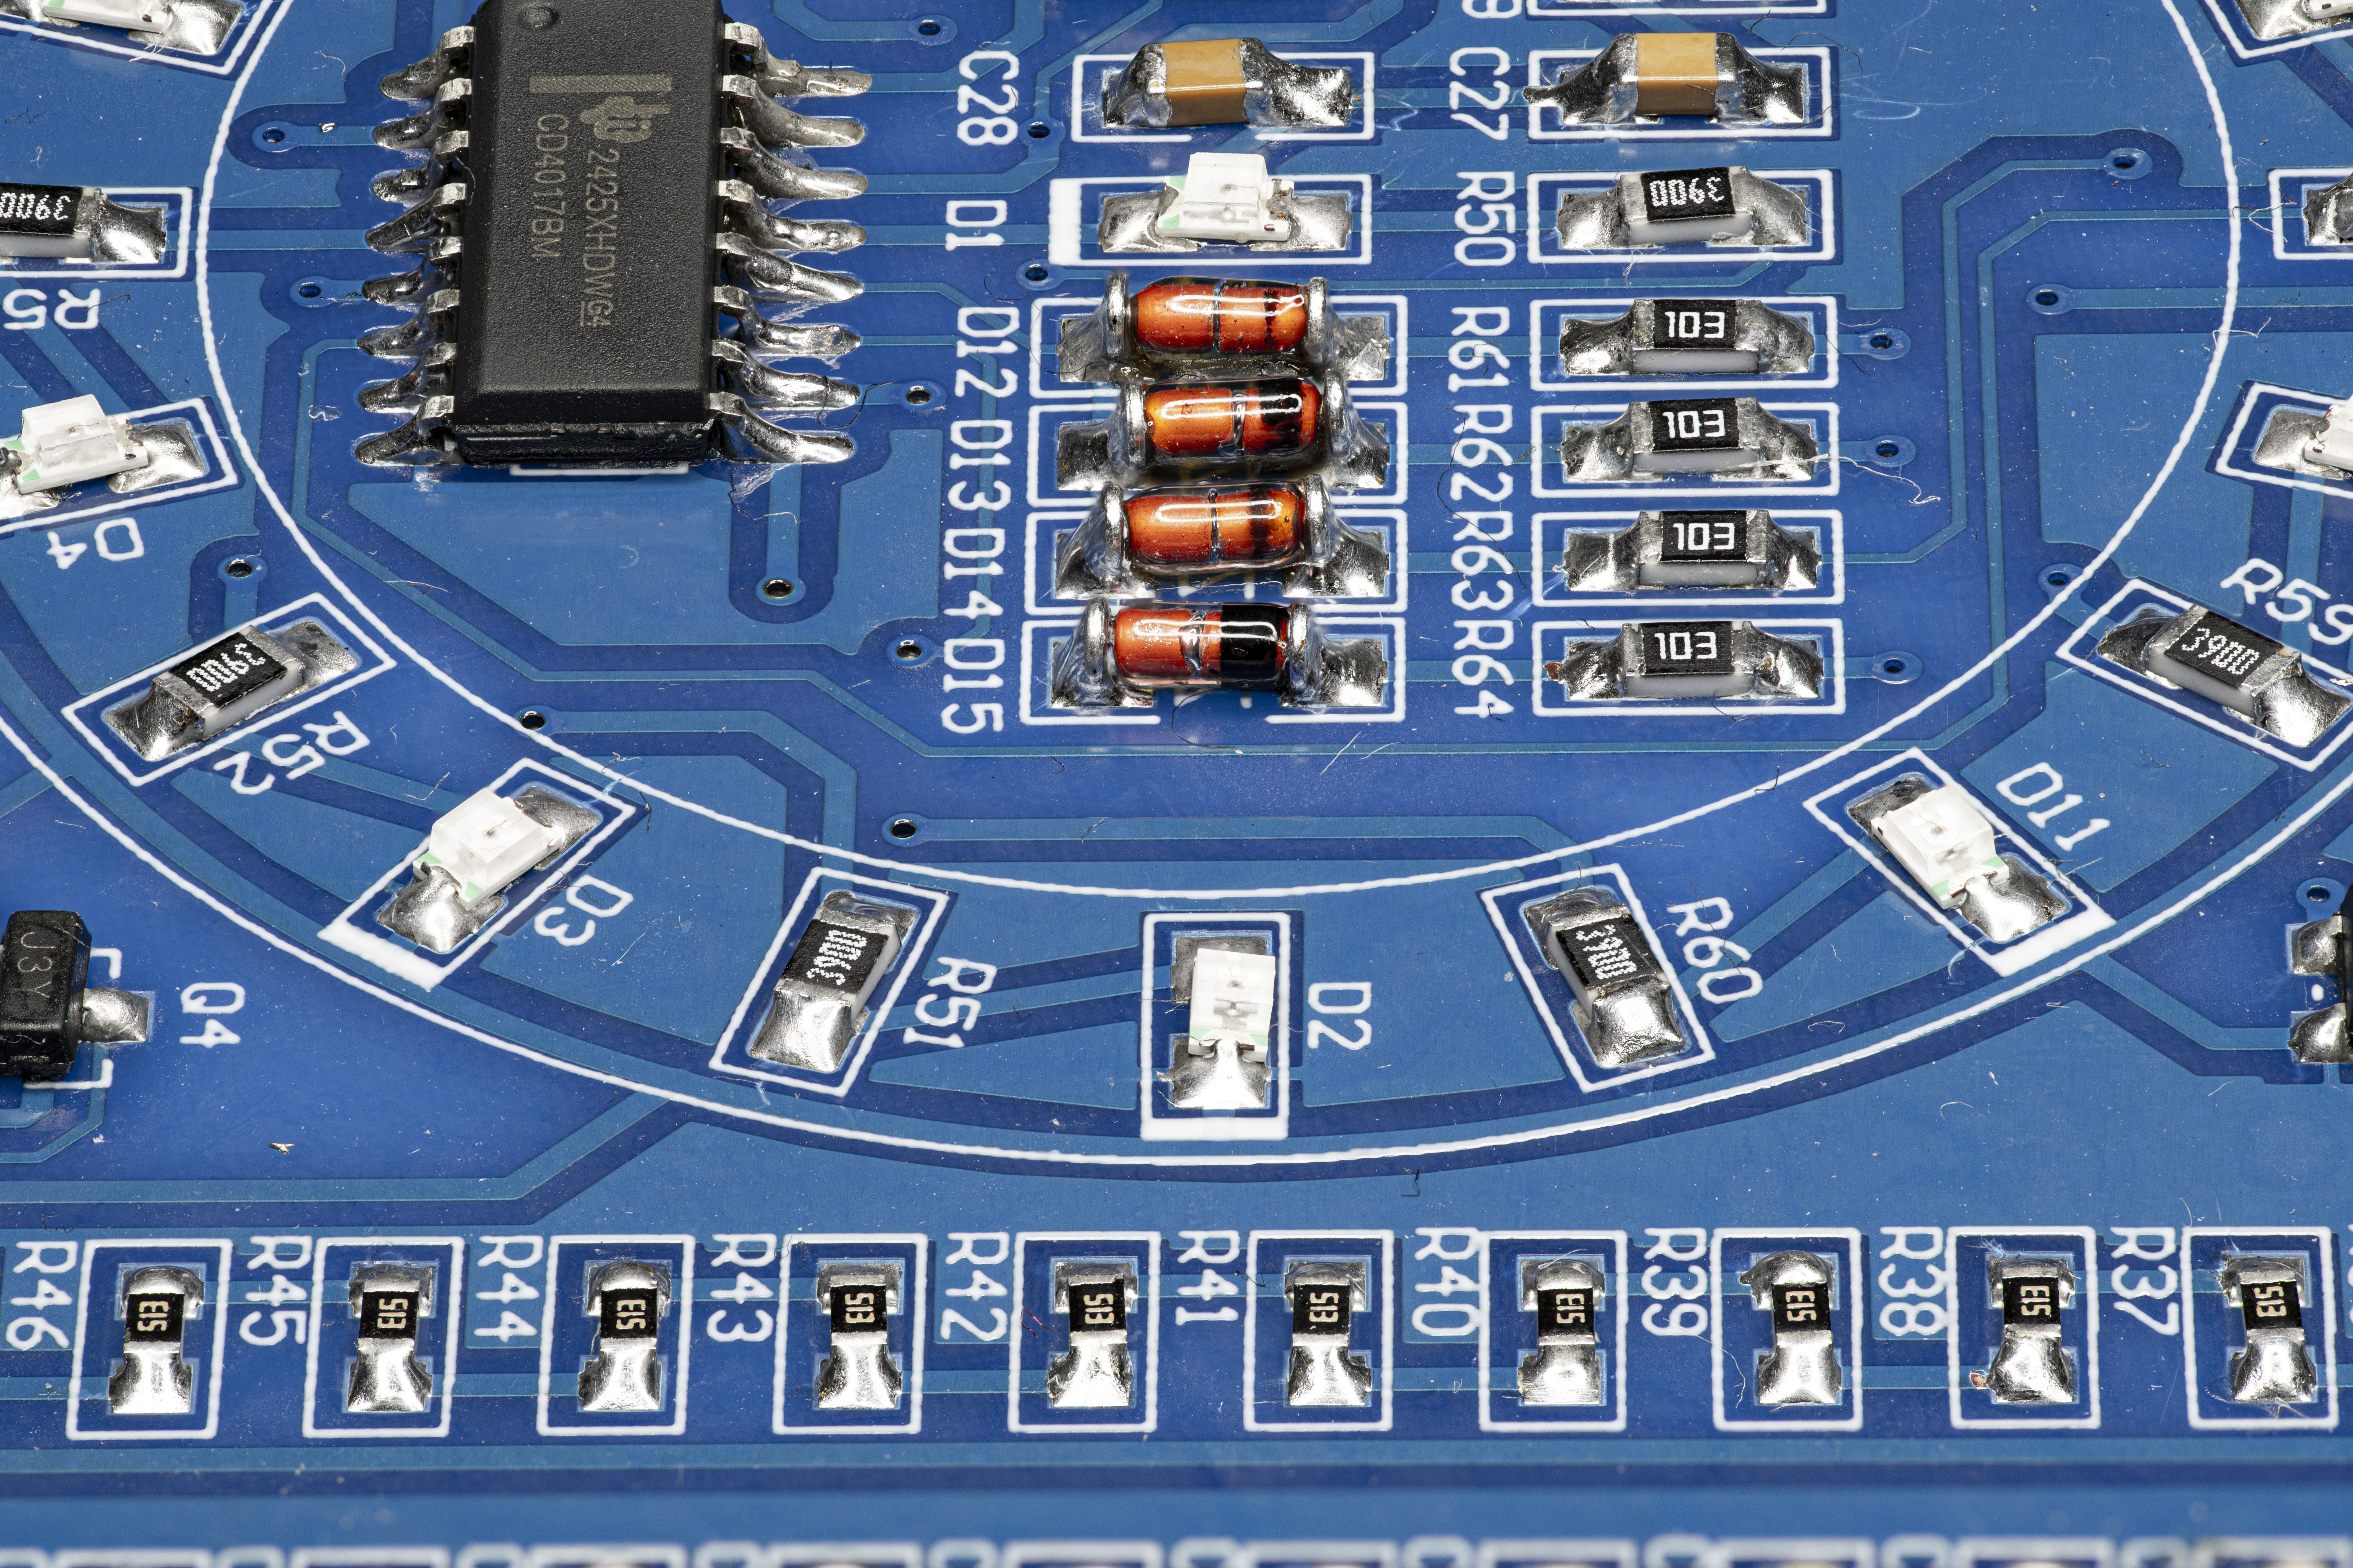
\includegraphics[width=\linewidth,keepaspectratio]{2.0.0.0_content/assets/bilder/smd platine nahaufname seitlich.jpg}
    \end{column}
\end{columns}
\end{frame}

\begin{frame}{Elektrische Prüfung}
\begin{columns}[T]
    \begin{column}{0.58\textwidth}
        \small
        \begin{itemize}\setlength{\itemsep}{3mm}
            \item Mit einem Messgerät kann man den \textbf{Durchgang} einer Verbindung prüfen.
            \item Ebenso lässt sich kontrollieren, ob irgendwo ein \textbf{Kurzschluss} entstanden ist.
            \item Gerade bei Fehlern lohnt sich diese Prüfung zusätzlich zur Sichtkontrolle.
        \end{itemize}
        \normalsize
    \end{column}
    \begin{column}{0.42\textwidth}
        \centering
        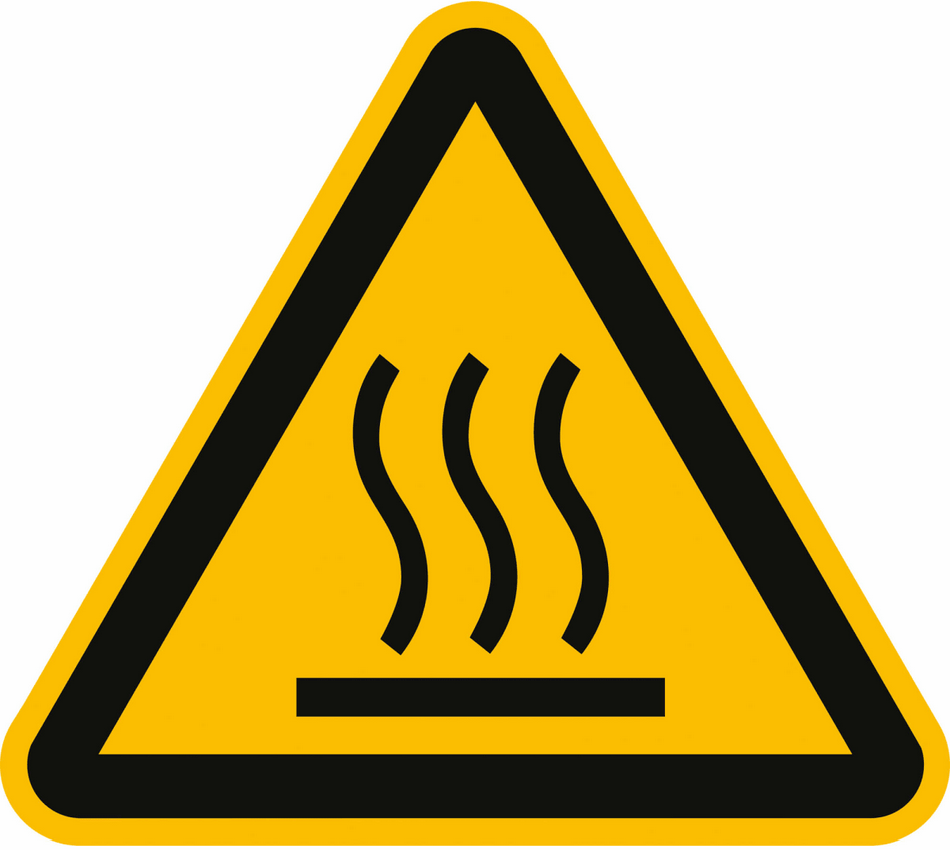
\includegraphics[width=\linewidth,keepaspectratio]{2.0.0.0_content/assets/bilder/Warnzeichen.png}
    \end{column}
\end{columns}
\end{frame}

\begin{frame}{Ablauf Praxis}
\begin{columns}[T]
    \begin{column}{0.58\textwidth}
        \small
        \begin{itemize}\setlength{\itemsep}{3mm}
            \item Zuerst gibt es eine \textbf{kurze Demo} am Arbeitsplatz.
            \item Danach folgt eine \textbf{Testplatine} oder ein einfacher erster Versuch.
            \item Anschließend kannst du ein \textbf{Projekt löten} und mit nach Hause nehmen.
        \end{itemize}
        \normalsize
    \end{column}
    \begin{column}{0.42\textwidth}
        \centering
        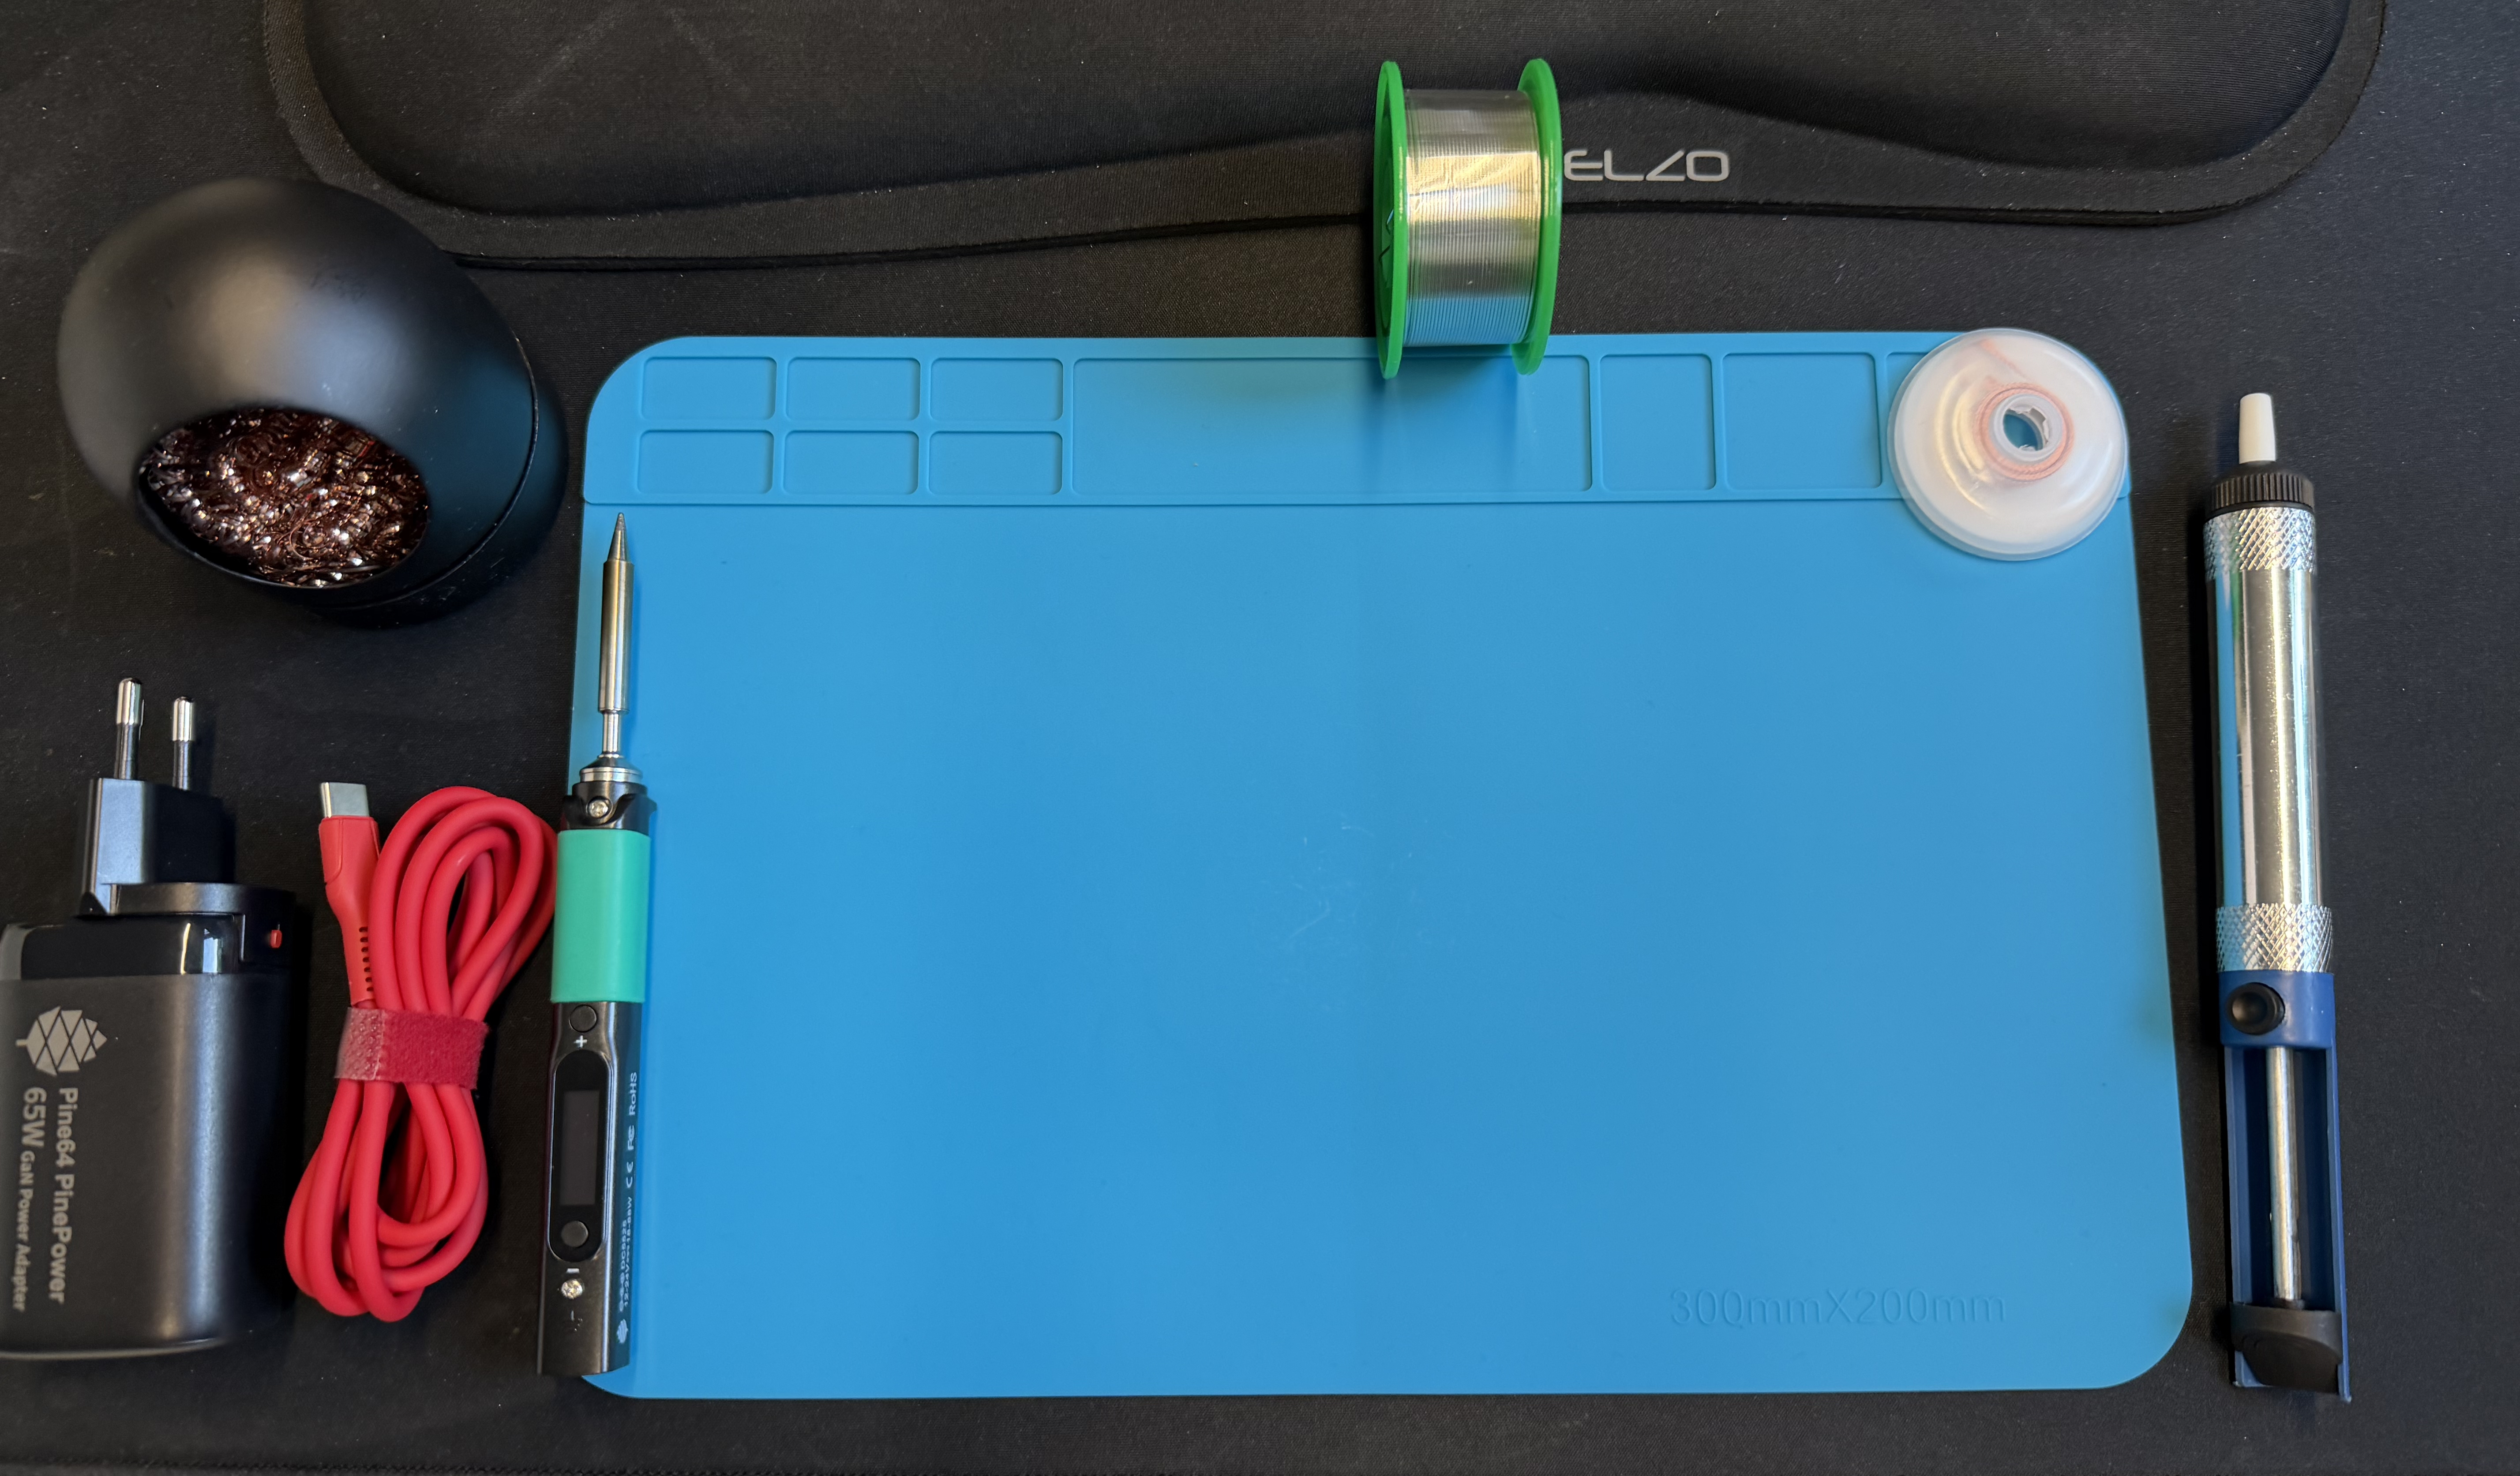
\includegraphics[width=\linewidth,keepaspectratio]{2.0.0.0_content/assets/bilder/setup.jpg}
    \end{column}
\end{columns}
\end{frame}

\begin{frame}{Merkhilfe}
\begin{itemize}\setlength{\itemsep}{3mm}
    \item \textbf{Wärme in die Verbindung}, nicht nur auf die Spitze
    \item \textbf{Zinn an das Werkstück}, nicht direkt an den Lötkolben
    \item \textbf{Ruhe beim Abkühlen}, damit die Lötstelle sauber aushärten kann
\end{itemize}
\end{frame}